\section{Performance}
\label{sec:performance}

We study the performance of the MEM in terms of the separation achieved between the $\dihiggs$ signal and the $\ttbar$ background
in terms of the LR $P(\vecy)$ given by Eq.~(\ref{eq:memLR}).
The separation is studied using samples of signal and background events produced by Monte Carlo (MC) simulation.
We study the separation for events simulated at LO and at NLO accuracy in pQCD.
The LO and NLO $\dihiggs$ signal samples each contain about fifty thousand events
and the LO and NLO $\ttbar$ background samples each contain about one million events.
All samples simulated at LO accuracy in pQCD are produced with the program $\textsc{MadGraph\_aMCatNLO}$ $2.2.2$,
while the samples simulated at NLO accuracy in pQCD are produced using the program $\textsc{POWHEG}$ $v2$~\cite{POWHEG1,POWHEG2,POWHEG3,POWHEGTTBAR1,POWHEGTTBAR2,POWHEGHH1,POWHEGHH2}.
The \textrm{NNPDF3.0} LO set of PDF is used for the simulation of the LO samples and the \textrm{NNPDF3.0} NLO set for the NLO samples~\cite{NNPDF1,NNPDF2,NNPDF3}.
Parton shower and hadronization processes are modeled using the program $\textsc{PYTHIA}$ $v8.2$~\cite{Sjostrand:2014zea} with the tune \textrm{CP5}~\cite{Sirunyan:2019dfx}.
All events are generated for proton-proton collisions at $\sqrt{s} = 13$~\TeV center-of-mass energy.
Events in which the electrons or muons originate from $\Pgt$ lepton decays,
\ie from the decay chains $\PW^{+} \to \Pgt^{+}\Pnu_{\Pgt} \to \Plepton^{+}\Pnu_{\Plepton}\APnu_{\Pgt}\Pnu_{\Pgt}$ or 
$\PW^{-} \to \Pgt^{-}\APnu_{\Pgt} \to \Plepton^{-}\APnu_{\Plepton}\Pnu_{\Pgt}\APnu_{\Pgt}$, are discarded.

We first study the events on MC-truth level, assuming that all measured observables $\vecy$ are equal to their true values.
This represents the case of an optimal experimental resolution and establishes the ideal performance that one can hope to achieve using the MEM.
We then study the effect of realistic experimental resolutions on the energy of $\Pbottom$-jets and on the momenta $\pX$ and $\pY$ of the hadronic recoil.
The case that one of the two reconstructed $\Pbottom$-jets is due to the misidentification of a light-quark or gluon jet,
while one of the true $\Pbottom$-jets fails to get reconstructed, is studied next.
The misidentification of a light-quark or gluon jet turns out to be the dominant experimental effect,
which limits the performance of the MEM.
We present an approach to mitigate the resulting loss in performance.
Next, we estimate the effect of using LO ME when computing the weights $w_{0}(\vecy)$ and $w_{1}(\vecy)$ 
by means of Eqs.~(\ref{eq:mem_signal}) and~(\ref{eq:mem_background}).
Unfortunately, we cannot compare the performance of the MEM
for the case of using ME generated at LO versus ME generated at NLO in Eqs.~(\ref{eq:mem_signal}) and~(\ref{eq:mem_background}) directly,
because the program $\textsc{MadGraph\_aMCatNLO}$ does not support the generation of code for NLO ME at present
and also because the usage of NLO ME in the MEM would increase the computing-time requirements by $1$-$2$ orders of magnitude.
Instead, we use ME generated at LO accuracy in Eqs.~(\ref{eq:mem_signal}) and~(\ref{eq:mem_background}) 
and compare the resulting performance in separating the $\dihiggs$ signal from the $\ttbar$ background
for MC samples simulated at LO and at NLO accuracy in pQCD.
The NLO samples are expected to provide the more accurate modelling of real data and the LO samples are taken as a more or less precise approximation.
We take the difference in performance achieved by the MEM on the MC samples simulated at LO and at NLO accuracy
as an estimate for the loss in discrimination power that results from our choice of using LO ME and ignoring the effects of higher orders in the MEM.
The difference in performance is found to be rather small.
We conclude the section on the performance of the MEM with a discussion of the computing-time requirements of the MEM.
As we will discuss in more detail in Section~\ref{sec:computing_time_requirements}, the demand in computing time is challenging already when using ME generated at LO accuracy.


\subsection{Optimal experimental resolution}

The study of the MEM performance on MC-truth level implies that all measured values $\vecy$ are equal to their true values $\vecyhat$.
Note that the experimental resolution on the energy of $\Pbottom$-jets and on the hadronic recoil still enters via the choice of the TF $W(E|\Ehat)$ in Eq.~(\ref{eq:TF_b})
and of the matrix $V$ in Eq.~(\ref{eq:TF_hadRecoil}).
Our choice of the TF is motivated by the resolutions achieved by the ATLAS and CMS experiments at the LHC~\cite{Aaboud:2017aca,PRF-14-001,Aaboud:2018tkc,JME-17-001}.
For the function $W(E|\Ehat)$, which models the energy resolution of $\Pbottom$-jets,
we choose a normal distribution:
\begin{linenowrapper}
\begin{equation}
W(E|\Ehat) = \frac{1}{\sqrt{2 \pi \sigma_{\Pbottom}^{2}}} \, e^{-\frac{(E - \Ehat)^{2}}{2 \, \sigma_{\Pbottom}^{2}}} \, ,
\label{eq:resolution_b}
\end{equation}
\end{linenowrapper}
with a standard deviation $\sigma_{\Pbottom}$ of $\sigma_{\Pbottom} = 100\% \cdot \sqrt{\Ehat}$.
Concerning the resolution on the hadronic recoil,
we assume that the components $\pX^{\rho}$ and $\pY^{\rho}$ are each measured with a resolution of $\sigma_{\rho} = 10$~\GeV:
\begin{linenowrapper}
\begin{equation}
V = \sigma_{\rho}^{2} \cdot I_{2} \, .
\label{eq:resolution_rho}
\end{equation}
\end{linenowrapper}
Distributions in the LR $P(\vecy)$, computed for simulated $\dihiggs$ signal and $\ttbar$ background events on MC-truth level, are shown in Fig.~\ref{fig:memLR_and_ROC_unsmeared}.
Signal events are characterized by high values of $P(\vecy)$, while background events typically have low values.
The figure also presents the ``receiver-operating-characteristic'' (ROC) curve~\cite{ROCcurve} that corresponds to the shown distribution in $P(\vecy)$.
The ROC curve quantifies the separation between the $\dihiggs$ signal and the $\ttbar$ background
and is obtained by varying the threshold of a cut on $P(\vecy)$ and plotting the fractions of signal and background events passing the cut.
For a signal efficiency of $35\%$, the $\ttbar$ background is reduced by three orders of magnitude.

\begin{figure}
\ifx\ver\verPreprint
\setlength{\unitlength}{1mm}
\begin{center}
\begin{picture}(160,67)(0,0)
\put(-1.0, 1.0){\mbox{\includegraphics*[height=66mm]
 {plots/signal_vs_background_memLR_unsmeared.pdf}}}
\put(80.0, 0.0){\mbox{\includegraphics*[height=67mm]
 {plots/ROC_unsmeared.pdf}}}
\end{picture}
\end{center}
\fi
\ifx\ver\verPAPER
\centering
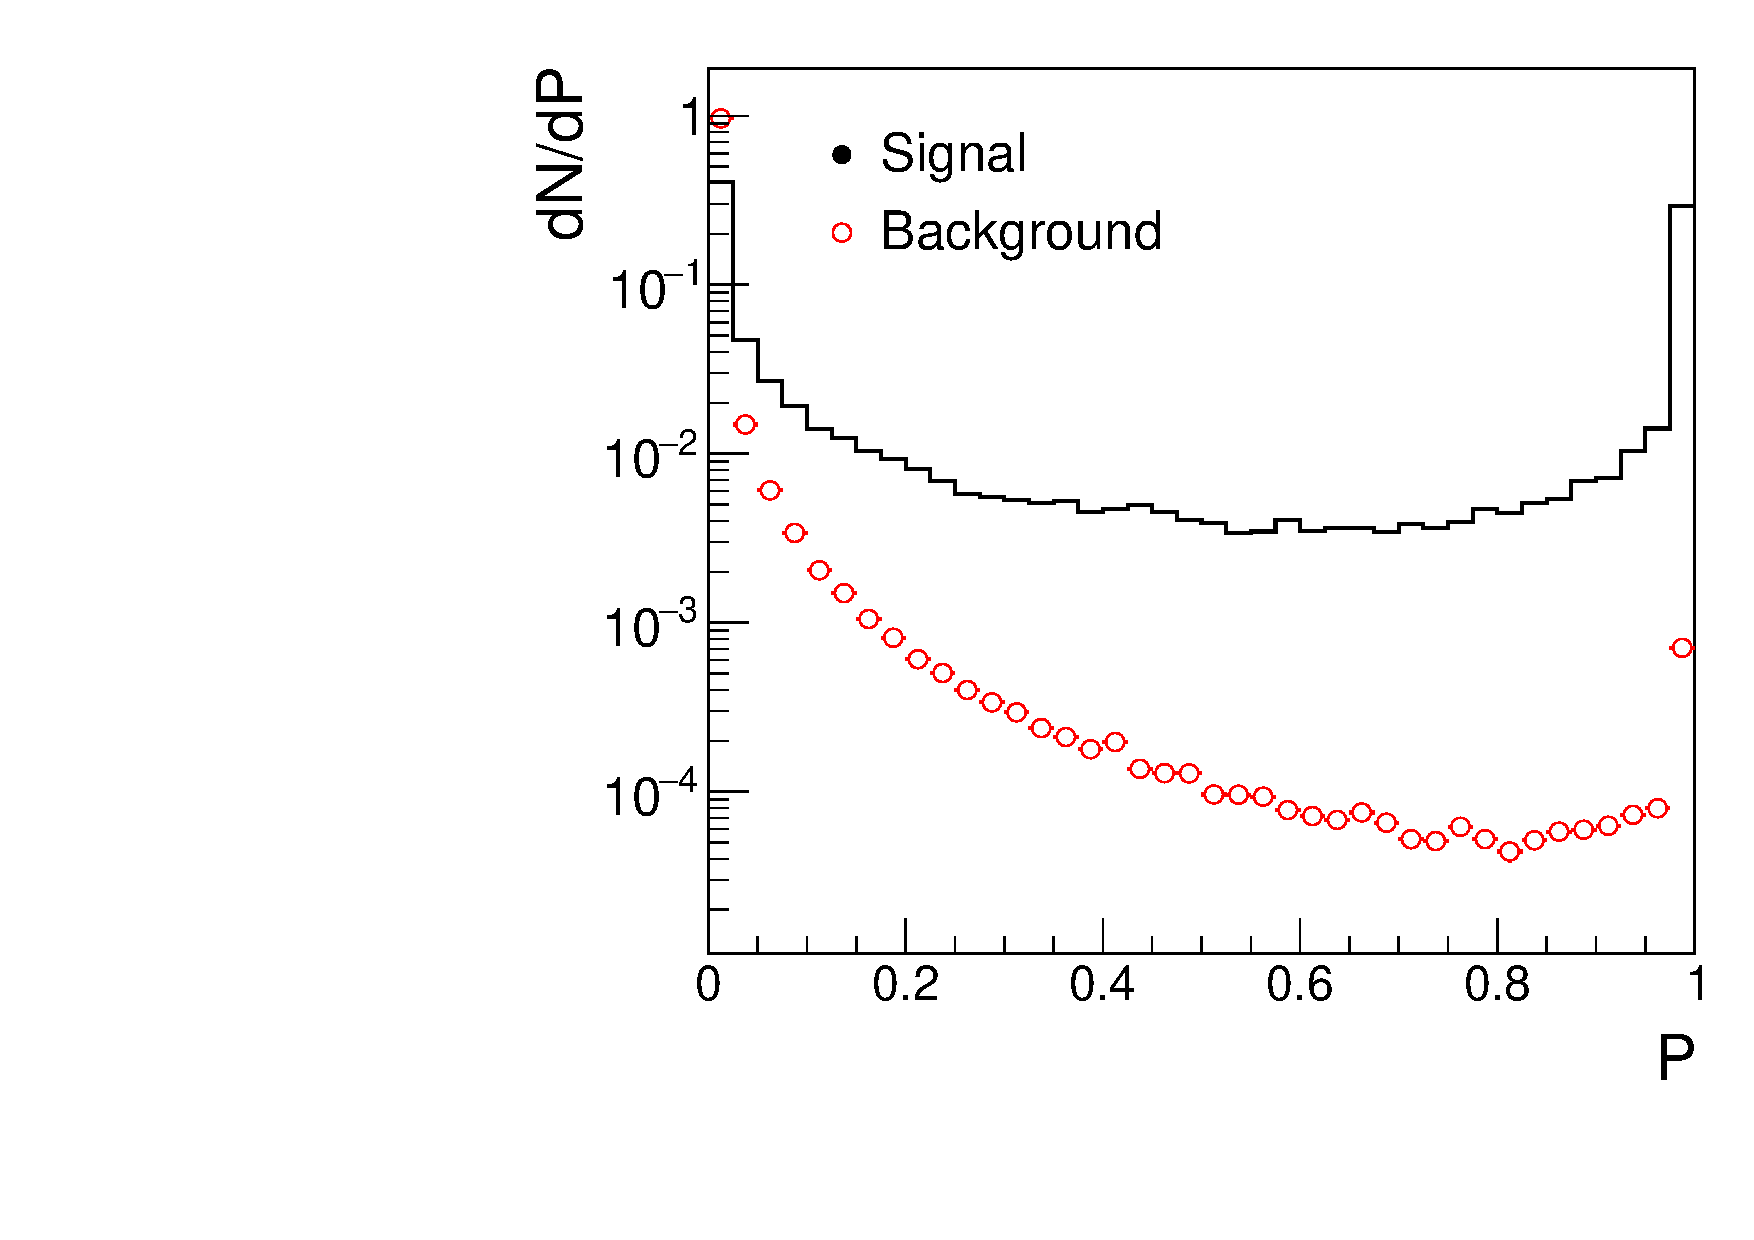
\includegraphics[width=0.48\textwidth]{plots/signal_vs_background_memLR_unsmeared.pdf}
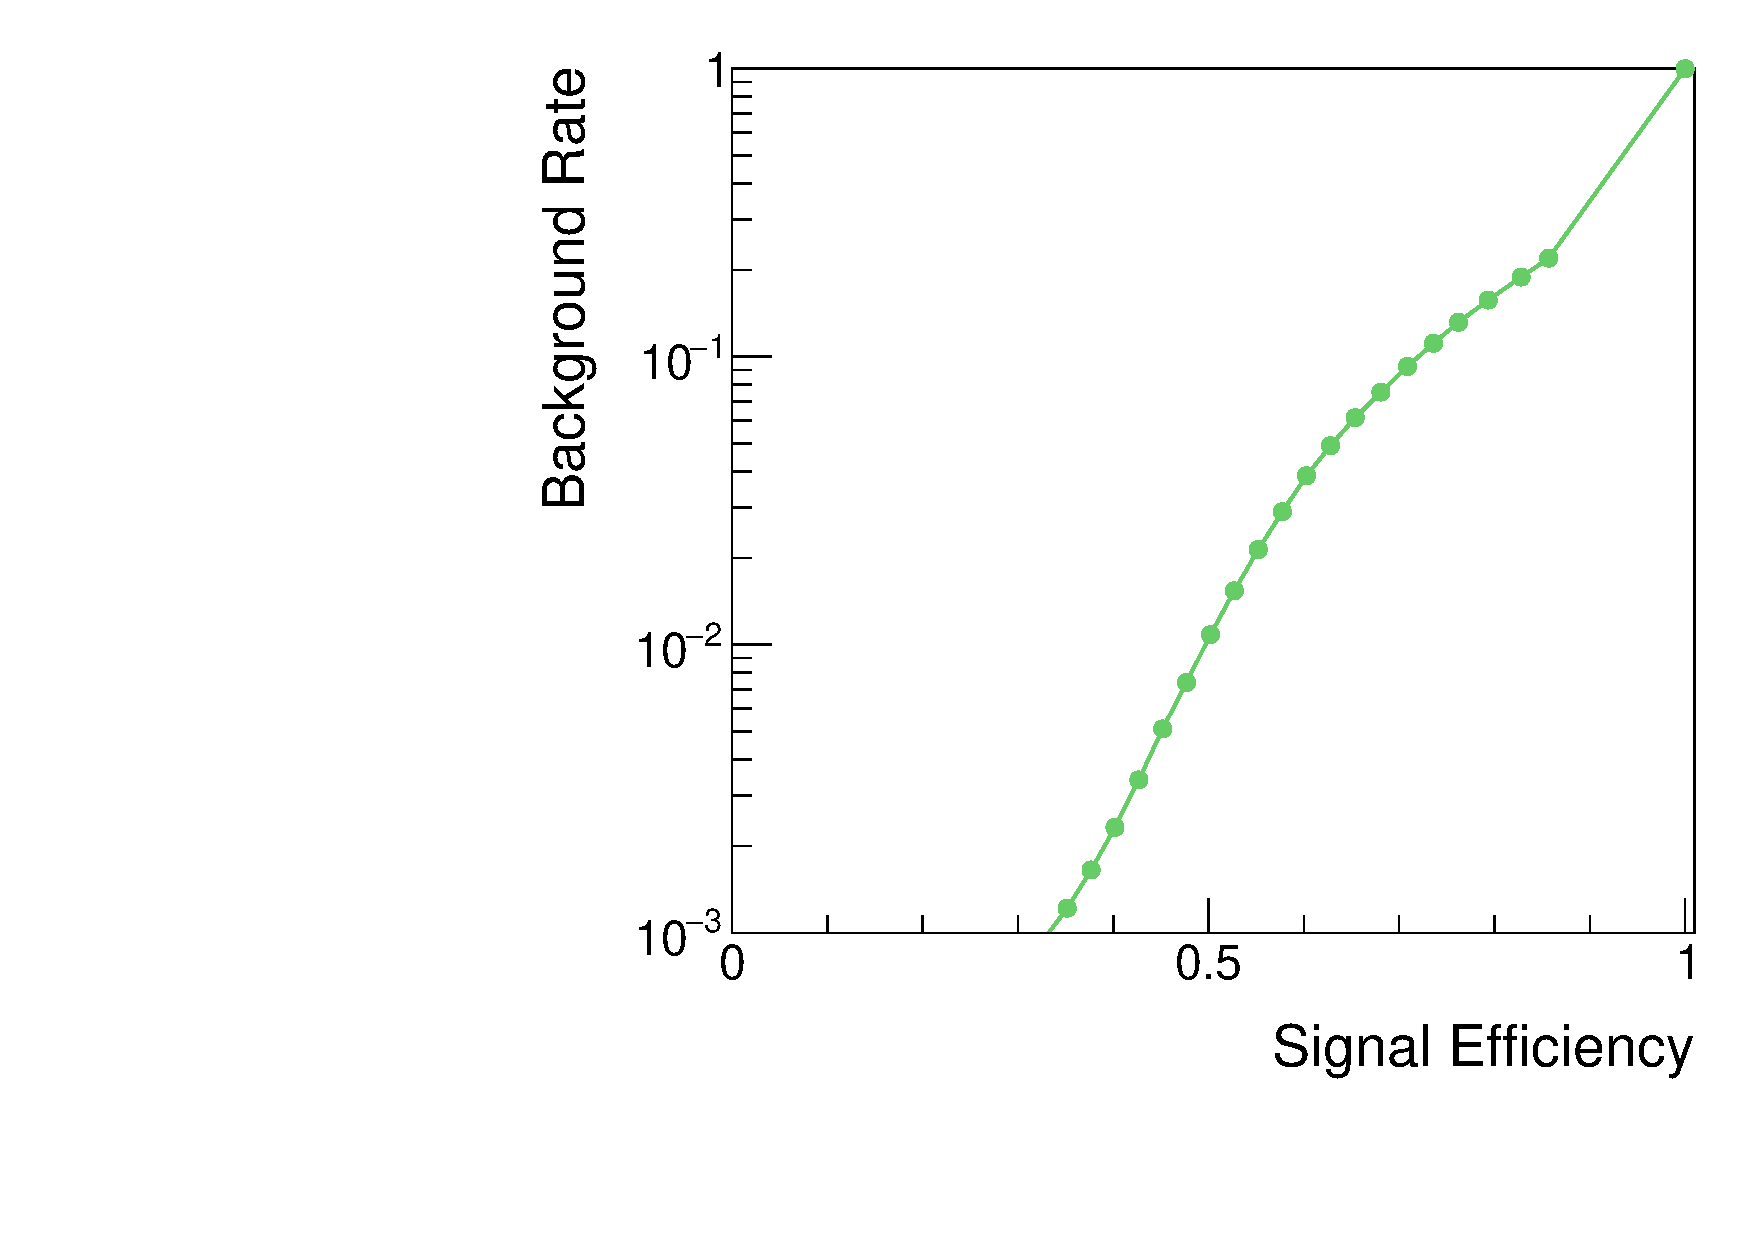
\includegraphics[width=0.48\textwidth]{plots/ROC_unsmeared.pdf}
\fi
\caption{
  Left: Distribution in the LR $P(\vecy)$ given by Eq.~(\ref{eq:memLR}), obtained for $\dihiggs$ signal and for $\ttbar$ background events.
  Right: Graph of background rate versus signal efficiency (``ROC curve''), obtained by applying a cut on the distribution shown on the left
  and varying the cut threshold.
  The signal and background events are studied on MC-truth level.
}
\label{fig:memLR_and_ROC_unsmeared}
\end{figure}

We will allude to this signal efficiency and background rejection in the following,
when quantifying the effect of the experimental resolution on the energy of $\Pbottom$-jets and on the hadronic recoil,
as well as of the misidentification of light-quark and gluon jets as $\Pbottom$-jets.


\subsection{Effect of experimental resolution on \texorpdfstring{$\Pbottom$}{b}-jets and hadronic recoil}

The effect of the experimental resolution on the distributions in the LR $P(\vecy)$ and on the ROC curve is estimated
by randomly sampling the energy $E$ of $\Pbottom$-jets and the components $\pX^{\rho}$ and $\pY^{\rho}$ of the hadronic recoil from the corresponding TF,
given by Eqs.~(\ref{eq:TF_b}) and~(\ref{eq:TF_hadRecoil}), and recomputing the LR $P(\vecy)$ for each such variation.
The resolutions on the energy of $\Pbottom$-jets and on the transverse momentum components of the hadronic recoil 
are given by Eqs.~(\ref{eq:resolution_b}) and~(\ref{eq:resolution_rho}).
The resulting distributions in $P(\vecy)$ are shown for $\dihiggs$ signal and $\ttbar$ background events in Fig.~\ref{fig:memLR_smeared}.
The distributions are compared to those obtained for the case that the LR $P(\vecy)$ is computed on MC-truth level.
The effect on the ROC curve is depicted in Fig.~\ref{fig:ROC_smeared}.
As one can see in the figure, the experimental resolution on the energy of $\Pbottom$-jets degrades the separation between the $\dihiggs$ signal and the $\ttbar$ background by a moderate amount
relative to the performance achieved on MC-truth level,
while the effect of the experimental resolution on the components $\pX^{\rho}$ and $\pY^{\rho}$ of the hadronic recoil is very small.

\begin{figure}
\ifx\ver\verPreprint
\setlength{\unitlength}{1mm}
\begin{center}
\begin{picture}(160,78)(0,0)
\put(0.0, 0.0){\mbox{\includegraphics*[height=78mm]
 {plots/effectOfSmearing_memLR_signal.pdf}}}
\put(81.0, 0.0){\mbox{\includegraphics*[height=78mm]
 {plots/effectOfSmearing_memLR_background.pdf}}}
\end{picture}
\end{center}
\fi
\ifx\ver\verPAPER
\centering
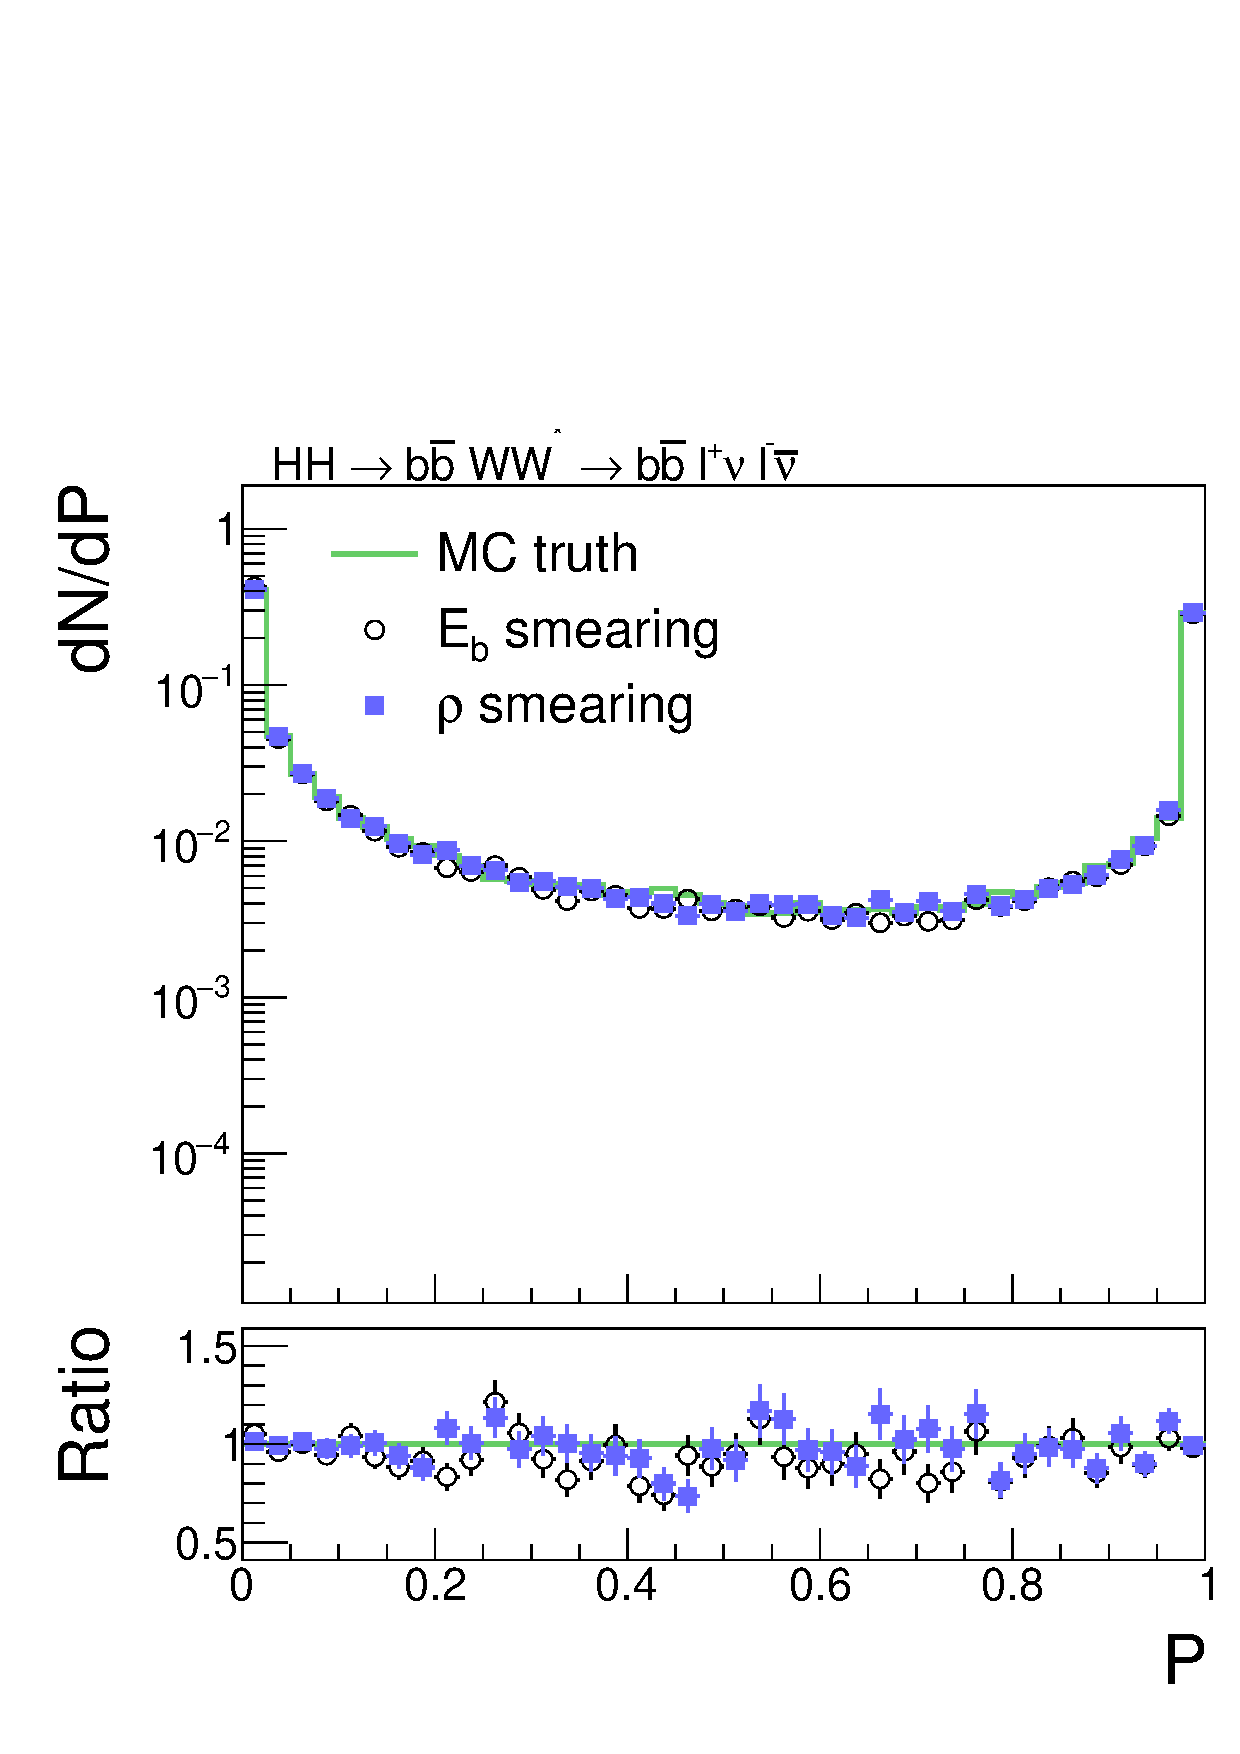
\includegraphics[width=0.48\textwidth]{plots/effectOfSmearing_memLR_signal.pdf}
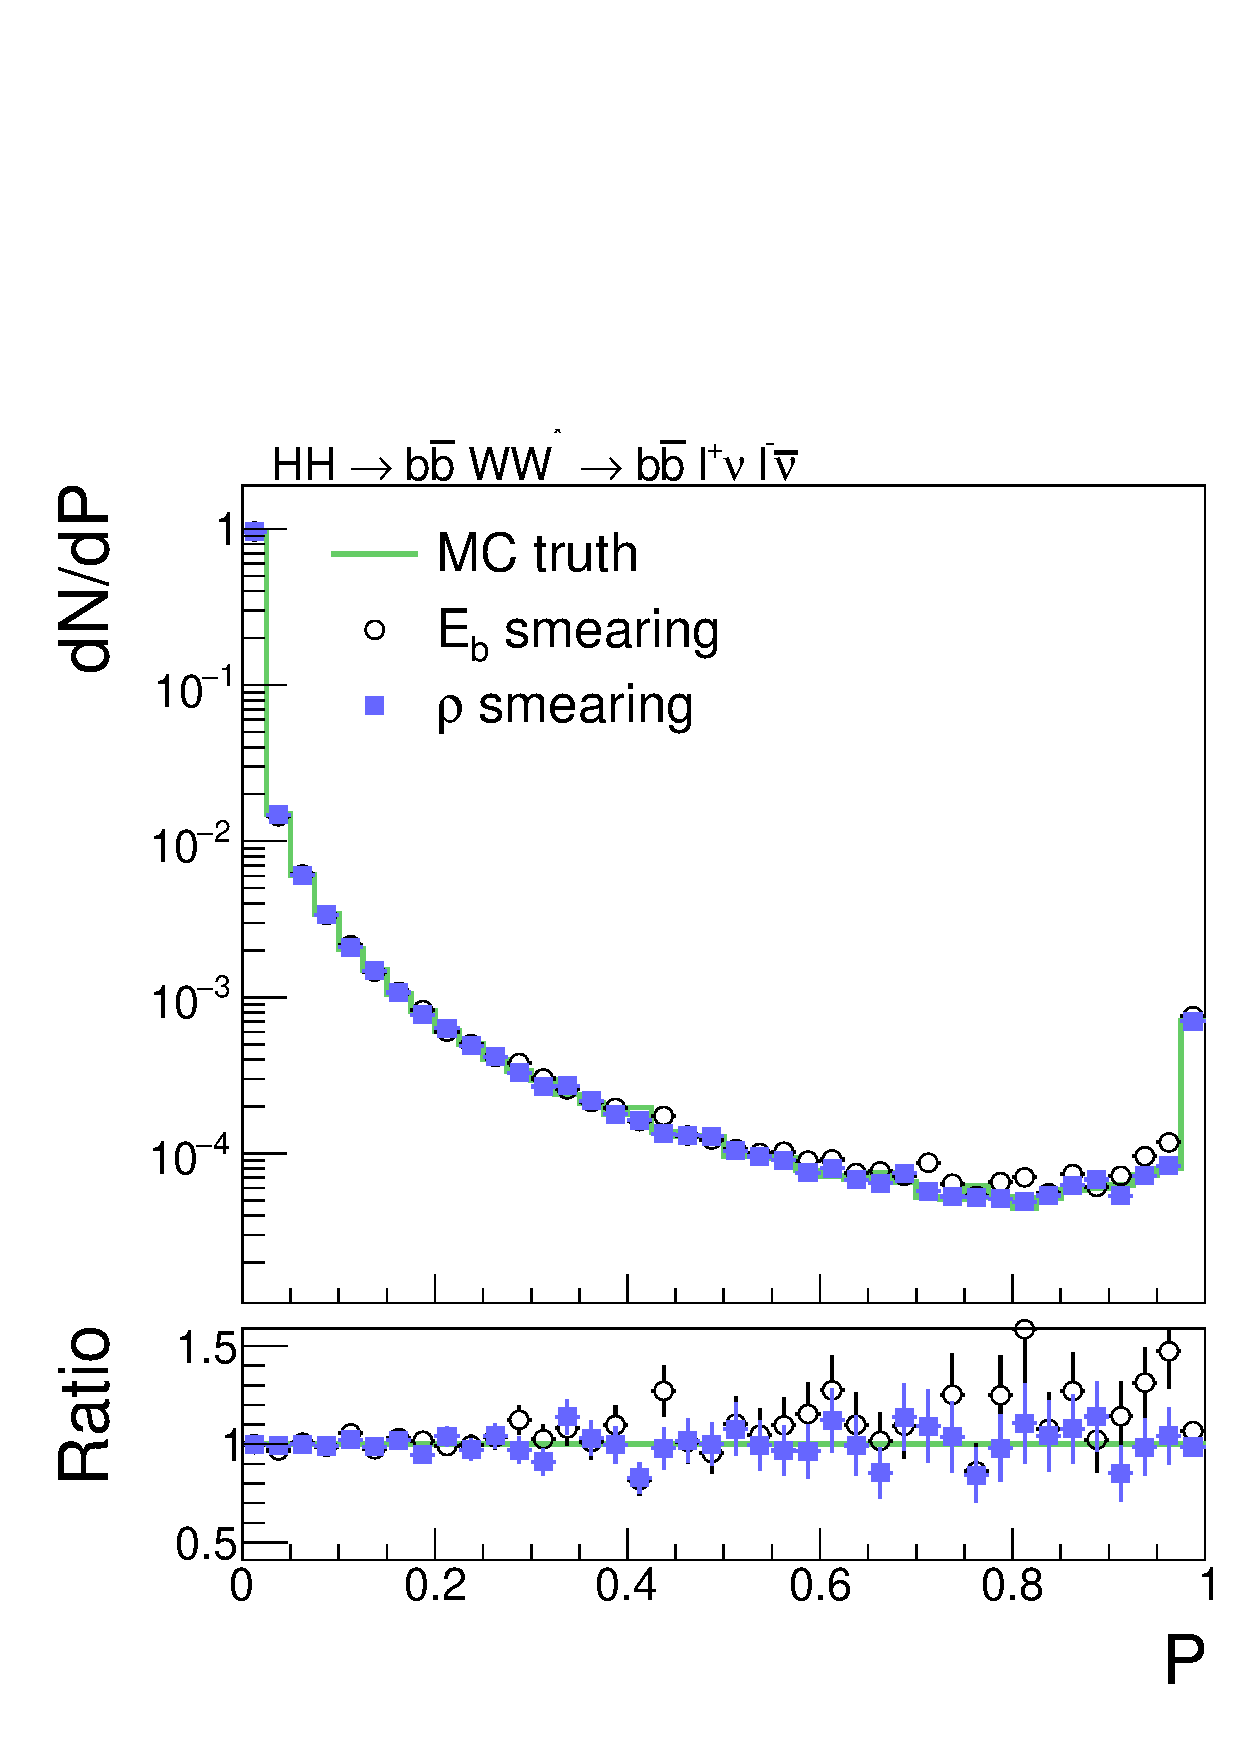
\includegraphics[width=0.48\textwidth]{plots/effectOfSmearing_memLR_background.pdf}
\fi
\caption{
  Effect of the experimental resolutions on the energy of $\Pbottom$-jets (``$E_{\Pbottom}$ smearing'') and on the hadronic recoil (``$\rho$ smearing'') 
  on the distribution in the LR $P(\vecy)$ obtained for simulated $\dihiggs$ signal (left) and $\ttbar$ background (right) events.
}
\label{fig:memLR_smeared}
\end{figure}

\begin{figure}
\ifx\ver\verPreprint
\setlength{\unitlength}{1mm}
\begin{center}
\begin{picture}(160,78)(0,0)
\put(39.5, 0.0){\mbox{\includegraphics*[height=78mm]
 {plots/effectOfSmearing_ROC.pdf}}}
\end{picture}
\end{center}
\fi
\ifx\ver\verPAPER
\centering
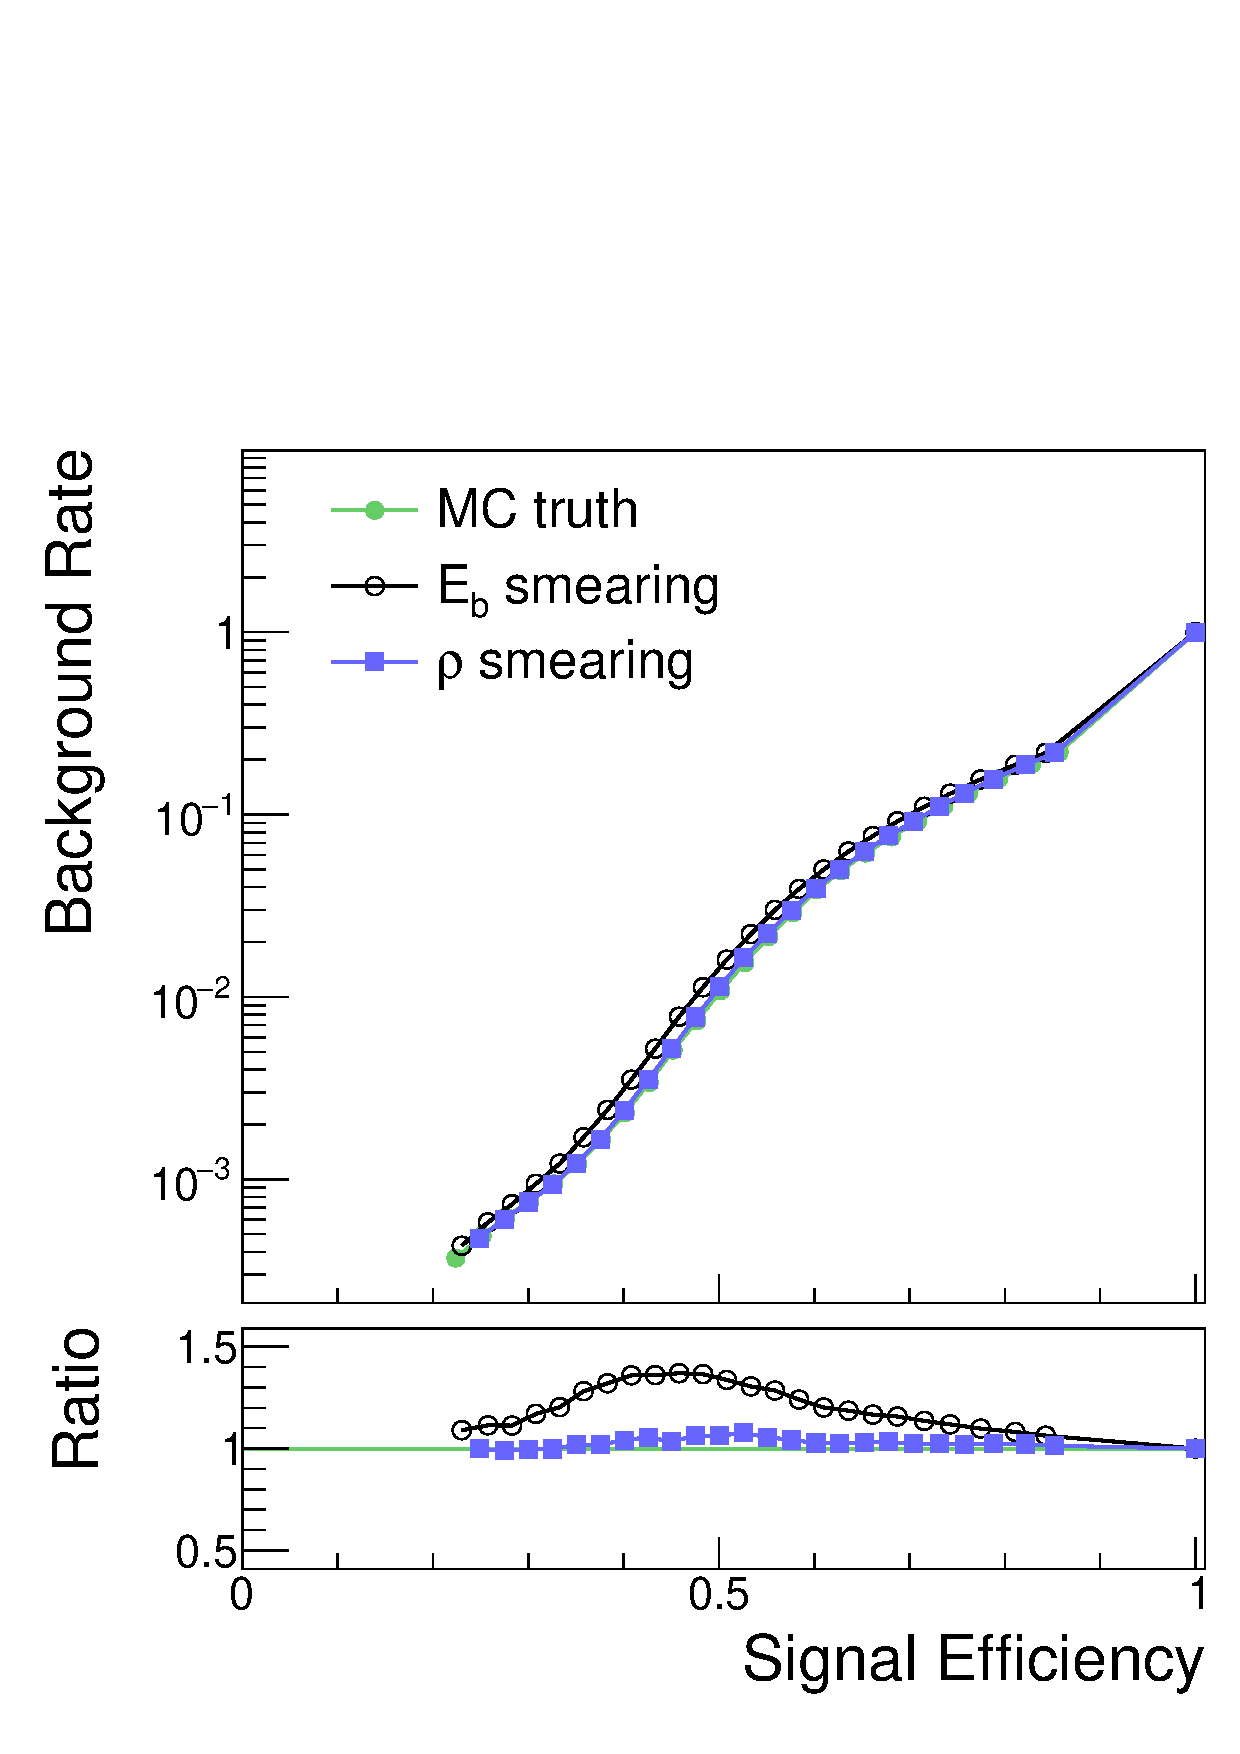
\includegraphics[width=0.48\textwidth]{plots/effectOfSmearing_ROC.pdf}
\fi
\caption{
  Effect of the experimental resolutions on the energy of $\Pbottom$-jets (``$E_{\Pbottom}$ smearing'') and on the hadronic recoil (``$\rho$ smearing'') 
  on the ROC curve. 
}
\label{fig:ROC_smeared}
\end{figure}


\subsection{Effect of misidentifying light-quark and gluon jets as \texorpdfstring{$\Pbottom$}{b}-jets}

Besides the experimental resolution on the $\Pbottom$-jet energy and on the hadronic recoil,
reconstruction effects may degrade the separation between the $\dihiggs$ signal and the $\ttbar$ background
in case one of the two $\Pbottom$-jets that are produced in the decays of the $\PHiggs$ boson or of the top quark pair
fails to get reconstructed,
and a light-quark or gluon jet gets misidentified as $\Pbottom$-jet.
The light-quark or gluon jet can be produced by either ISR or final-state radiation (FSR), from the underlying event, 
or from additional proton-proton interactions (pileup) occurring in the same bunch-crossing as the hard-scattering interaction.
The efficiency to identify $\Pbottom$-jets typically amounts to $60$-$70\%$ at the ATLAS and CMS experiments,
for a misidentification rate for light-quark and gluon jets of order $1\%$~\cite{Aad:2015ydr,BTV-16-002}.

We simulate the effect that one of the two true $\Pbottom$-jets fails to get reconstructed and a light-quark or gluon jet gets misidentified as $\Pbottom$-jet
by replacing $10\%$ of true $\Pbottom$-jets by randomly selected light-quark or gluon jets produced by either ISR or FSR, or from the underlying event 
(our simulated samples of signal and background events do not include pileup). 
We then compare the distributions in the LR $P(\vecy)$ thus obtained with the corresponding distributions obtained for the case that both $\Pbottom$-jets are genuine $\Pbottom$-jets.
The results are shown in Fig.~\ref{fig:memLR_fakeBJet}.
We observe that the misidentification of light-quark and gluon jets as $\Pbottom$-jets has a sizeable effect on the LR $P(\vecy)$.
More specifically, the distribution in $P(\vecy)$ obtained for signal events becomes significantly more background-like
in case a light-quark or gluon jet is misidentified as $\Pbottom$-jet.
Similarly, the distribution in $P(\vecy)$ obtained for background events becomes significantly more signal-like.
As a result, the separation between the $\dihiggs$ signal and the $\ttbar$ background degrades significantly,
resulting in a sizeable loss in performance of the MEM, whenever a light-quark or gluon jet is misidentified as $\Pbottom$-jet.
The loss in performance can be seen clearly in the ROC curve, which is shown in Fig.~\ref{fig:ROC_fakeBJet}.

\begin{figure}
\ifx\ver\verPreprint
\setlength{\unitlength}{1mm}
\begin{center}
\begin{picture}(160,66)(0,0)
\put(-1.0, 0.0){\mbox{\includegraphics*[height=66mm]
 {plots/effectOfFakes_2histograms_memLR_signal.pdf}}}
\put(80.0, 0.0){\mbox{\includegraphics*[height=66mm]
 {plots/effectOfFakes_2histograms_memLR_background.pdf}}}
\end{picture}
\end{center}
\fi
\ifx\ver\verPAPER
\centering
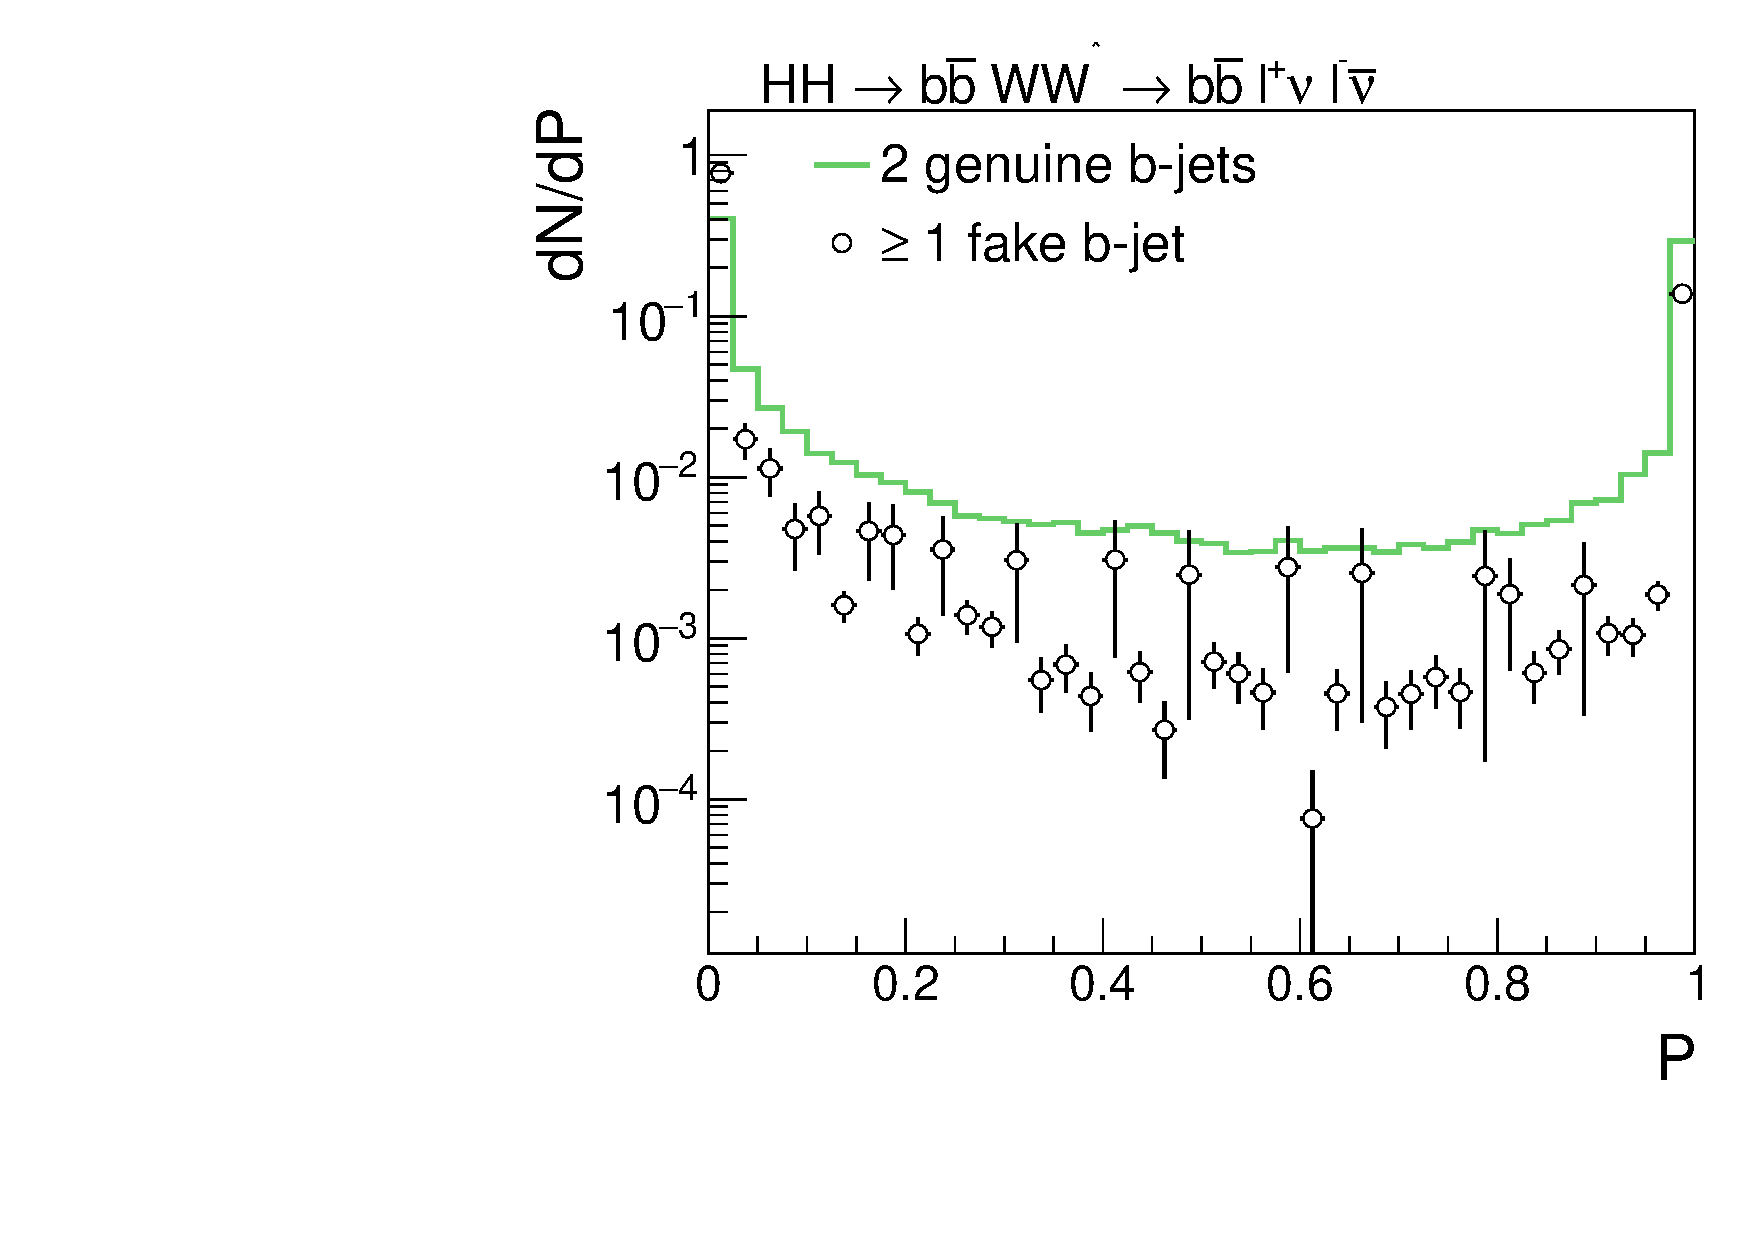
\includegraphics[width=0.48\textwidth]{plots/effectOfFakes_2histograms_memLR_signal.pdf}
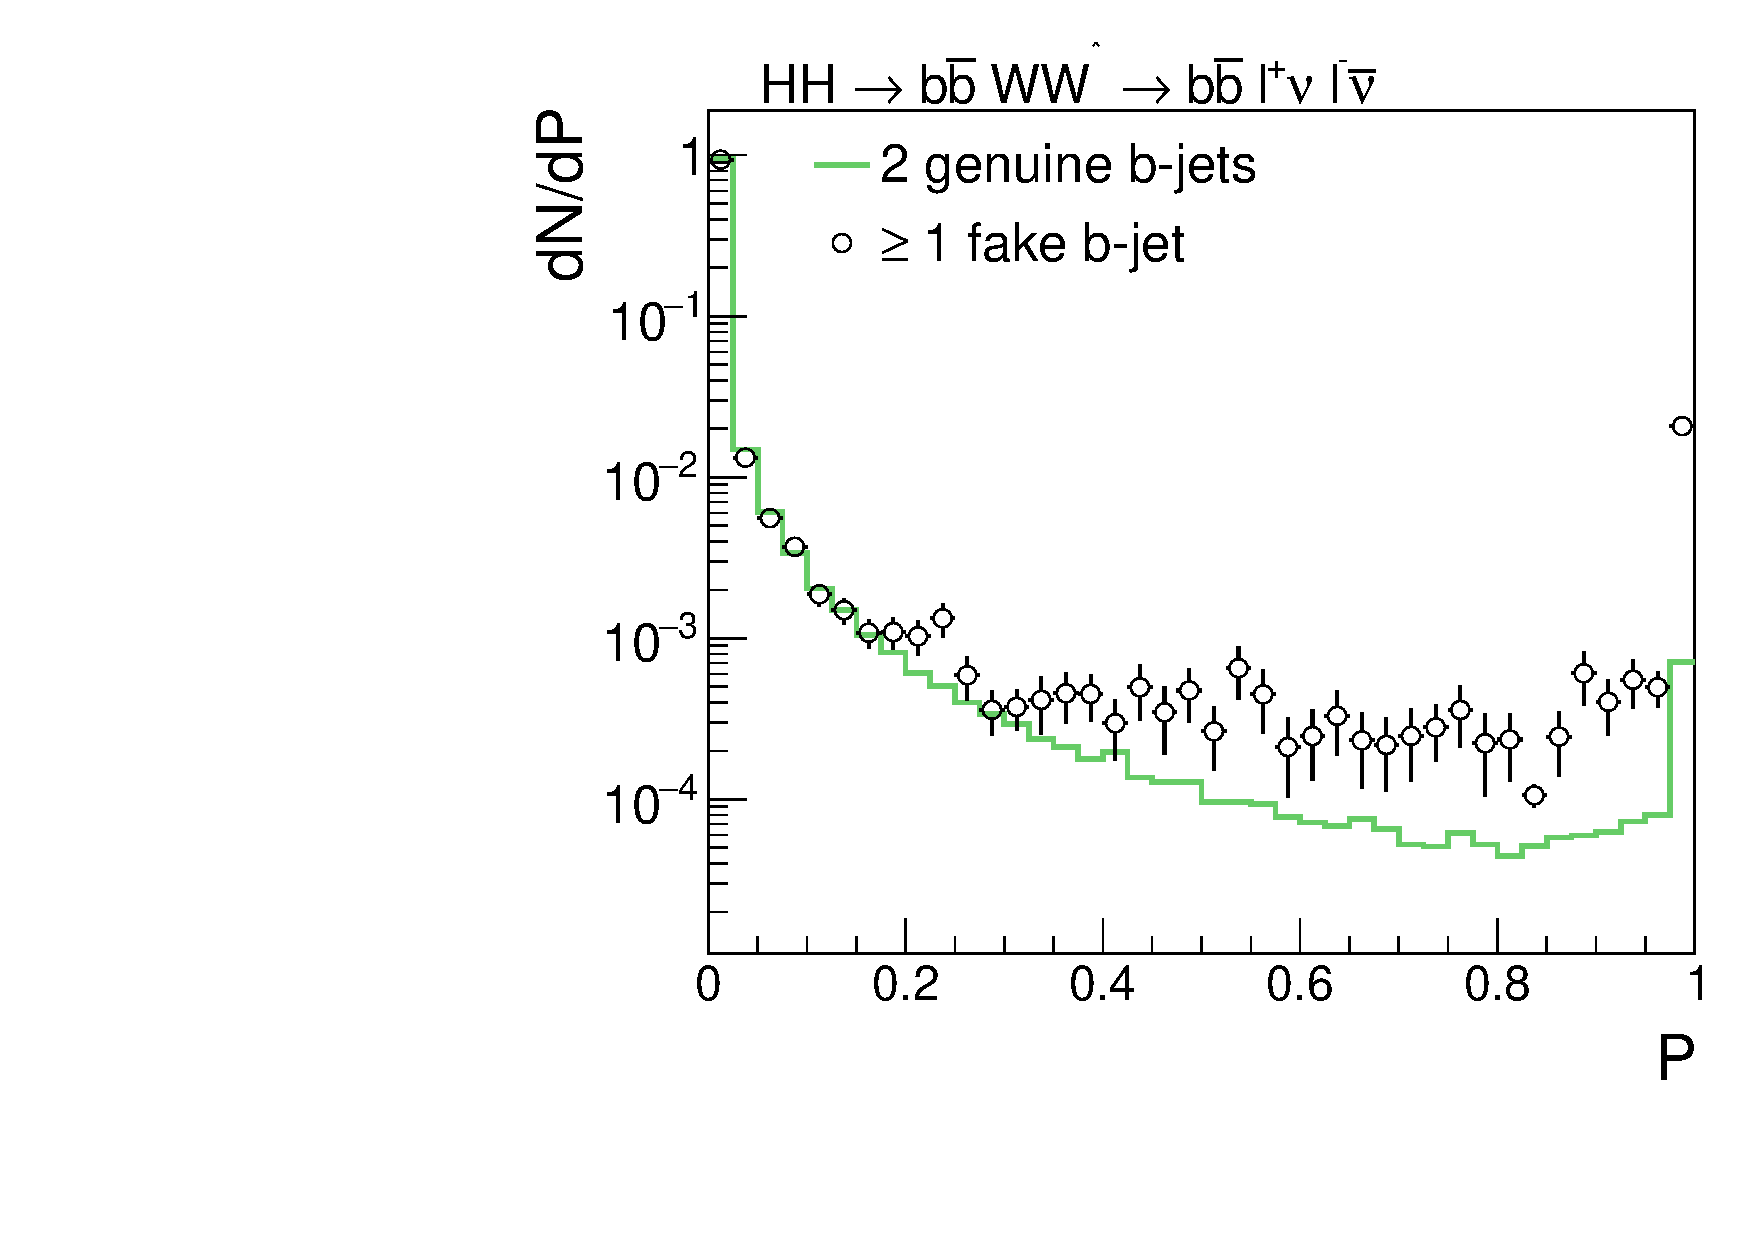
\includegraphics[width=0.48\textwidth]{plots/effectOfFakes_2histograms_memLR_background.pdf}
\fi
\caption{
  Effect of misidentifying a light-quark or gluon jet (``fake'') as $\Pbottom$-jet
  on the distribution in the LR $P(\vecy)$ obtained for simulated $\dihiggs$ signal (left) and $\ttbar$ background (right) events.
}
\label{fig:memLR_fakeBJet}
\end{figure}

\begin{figure}
\ifx\ver\verPreprint
\setlength{\unitlength}{1mm}
\begin{center}
\begin{picture}(160,67)(0,0)
\put(39.5, 0.0){\mbox{\includegraphics*[height=67mm]
 {plots/effectOfFakes_2graphs_ROC.pdf}}}
\end{picture}
\end{center}
\fi
\ifx\ver\verPAPER
\centering
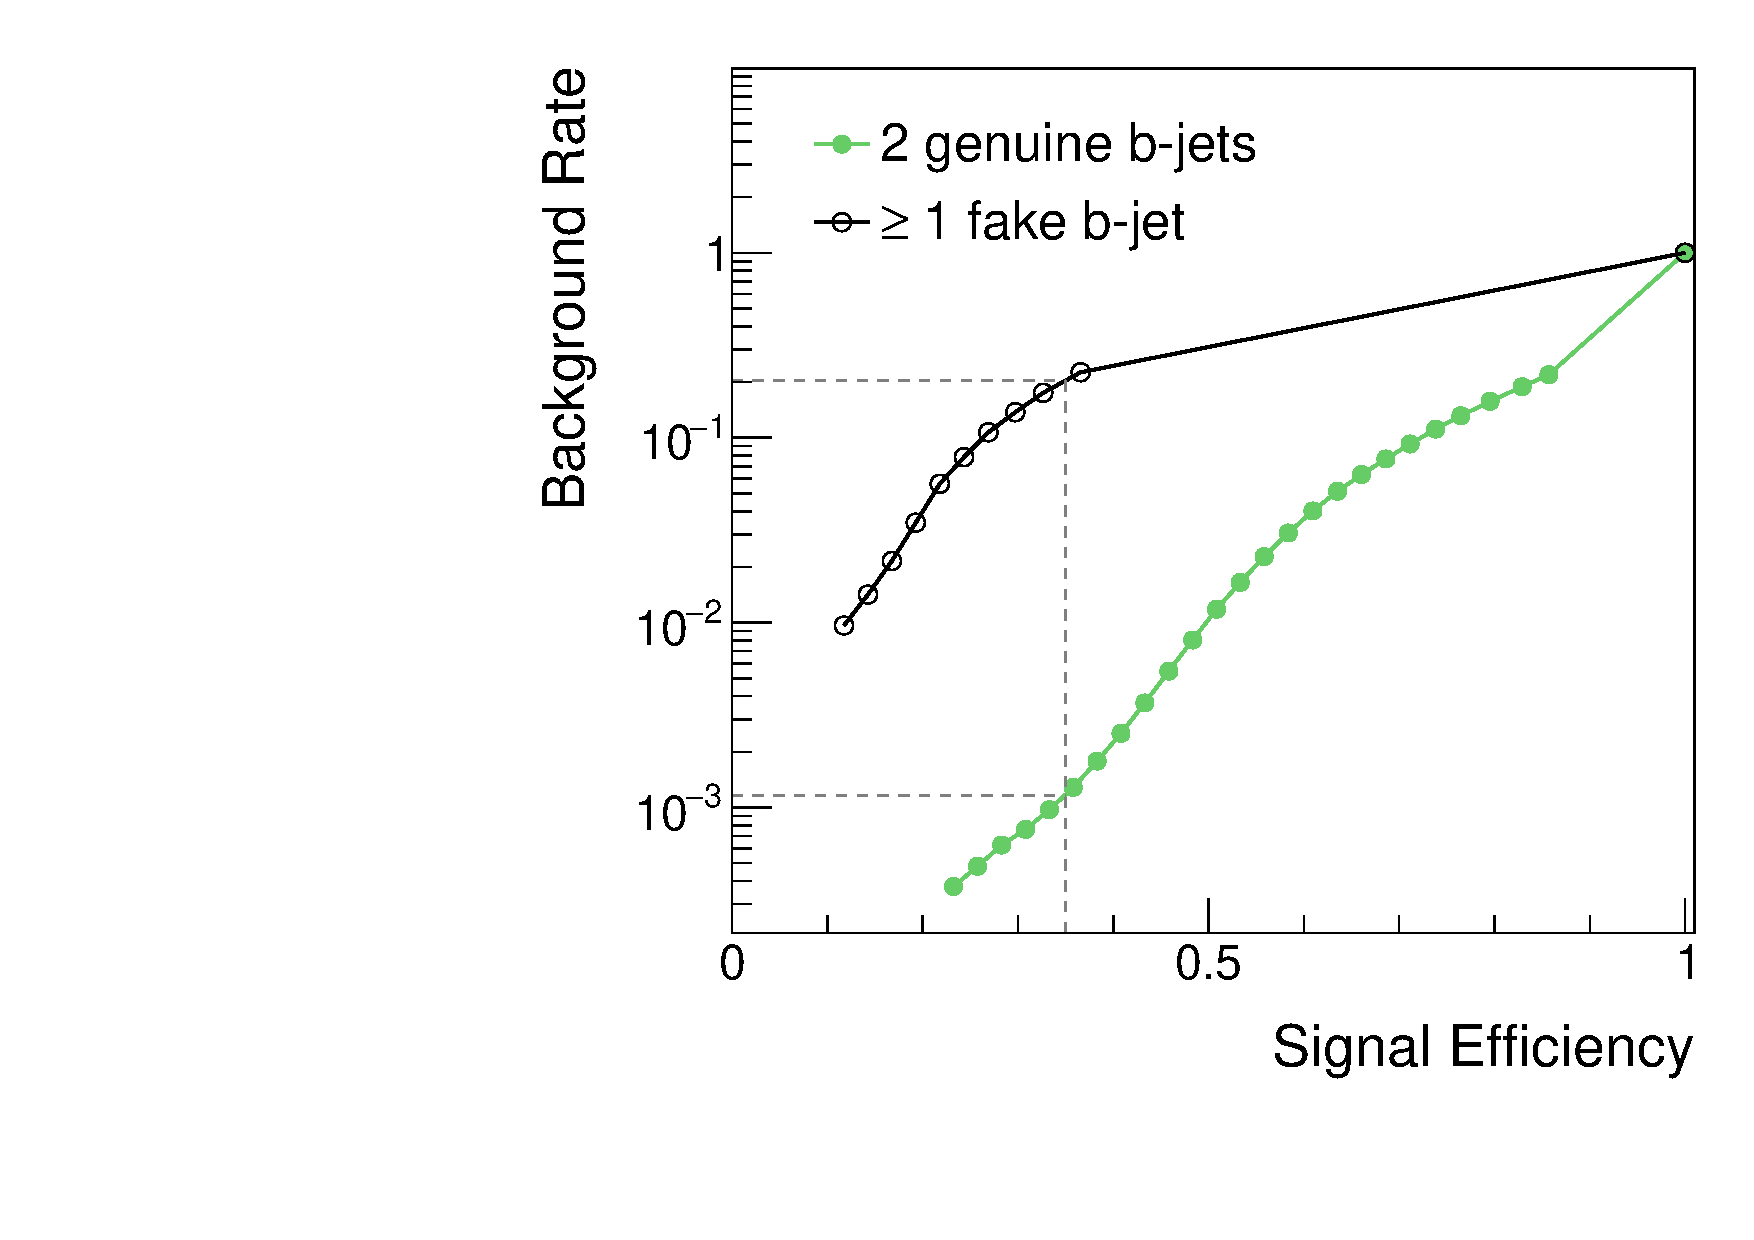
\includegraphics[width=0.48\textwidth]{plots/effectOfFakes_2graphs_ROC.pdf}
\fi
\caption{
  Effect of misidentifying a light-quark or gluon jet (``fake'') as $\Pbottom$-jet
  on the ROC curve.
}
\label{fig:ROC_fakeBJet}
\end{figure}

Compared to the effect of the experimental resolution on the $\Pbottom$-jet energy and on the momentum of the hadronic recoil,
the loss in signal-to-background separation arising from the misidentification of a light-quark or gluon jet as a $\Pbottom$-jet
is much more severe. 

The magnitude of the effect warrants further investigations concerning its origin and the development of approaches to mitigate the effect.
In Fig.~\ref{fig:probS_and_probB_fakeBJet} we show the distributions in the PDs $w_{0}(\vecy)$ and $w_{1}(\vecy)$
that quantify the level of compatibility with the signal and background hypotheses.
The distributions in $w_{0}(\vecy)$ and in $w_{1}(\vecy)$ are shown separately 
for signal and background events in which at least one of the two $\Pbottom$-jets is due to the misidentification of a light-quark or gluon jet
and for events in which both $\Pbottom$-jets are genuine $\Pbottom$-jets.
We observe that the distributions in the probability density for the ``correct'' hypothesis 
($w_{0}(\vecy)$ for signal and $w_{1}(\vecy)$ for background events)
are more susceptible to the misidentification of light-quark and gluon jets as $\Pbottom$-jets than the distributions in the PD for the ``wrong'' hypothesis 
($w_{1}(\vecy)$ for signal and $w_{0}(\vecy)$ for background events).
The distribution in the PD $w_{0}(\vecy)$ for signal events to be classified as signal is affected the most.
The large magnitude of the effect on $w_{0}(\vecy)$ is explained by the presence of a BW propagator in the ME $\mathcal{M}_{0}(\vecphat)$ for the signal hypothesis,
which enforces that the mass of the pair of $\Pbottom$-jets equals $m_{\PHiggs}$.
The $\delta$-function introduced into the integrand of Eq.~(\ref{eq:mem3}) via the transformations described in Section~\ref{sec:appendix_bEn_Hbb} of the appendix
guarantees the compliance with the $\PHiggs$ boson mass constraint,
but introduces large ``pulls'' in the TF $W(E|\Ehat)$ for the $\Pbottom$-jet energy,
in case a light-quark or gluon jet gets misidentified as $\Pbottom$-jet,
which diminish the value of the integrand.

\begin{figure}
\ifx\ver\verPreprint
\setlength{\unitlength}{1mm}
\begin{center}
\begin{picture}(160,144)(0,0)
\put(-1.0, 78.0){\mbox{\includegraphics*[height=66mm]
 {plots/effectOfFakes_2histograms_probS_signal.pdf}}}
\put(80.0, 78.0){\mbox{\includegraphics*[height=66mm]
 {plots/effectOfFakes_2histograms_probB_signal.pdf}}}
\put(-1.0, 0.0){\mbox{\includegraphics*[height=66mm]
 {plots/effectOfFakes_2histograms_probS_background.pdf}}}
\put(80.0, 0.0){\mbox{\includegraphics*[height=66mm]
 {plots/effectOfFakes_2histograms_probB_background.pdf}}}
\end{picture}
\end{center}
\fi
\ifx\ver\verPAPER
\centering
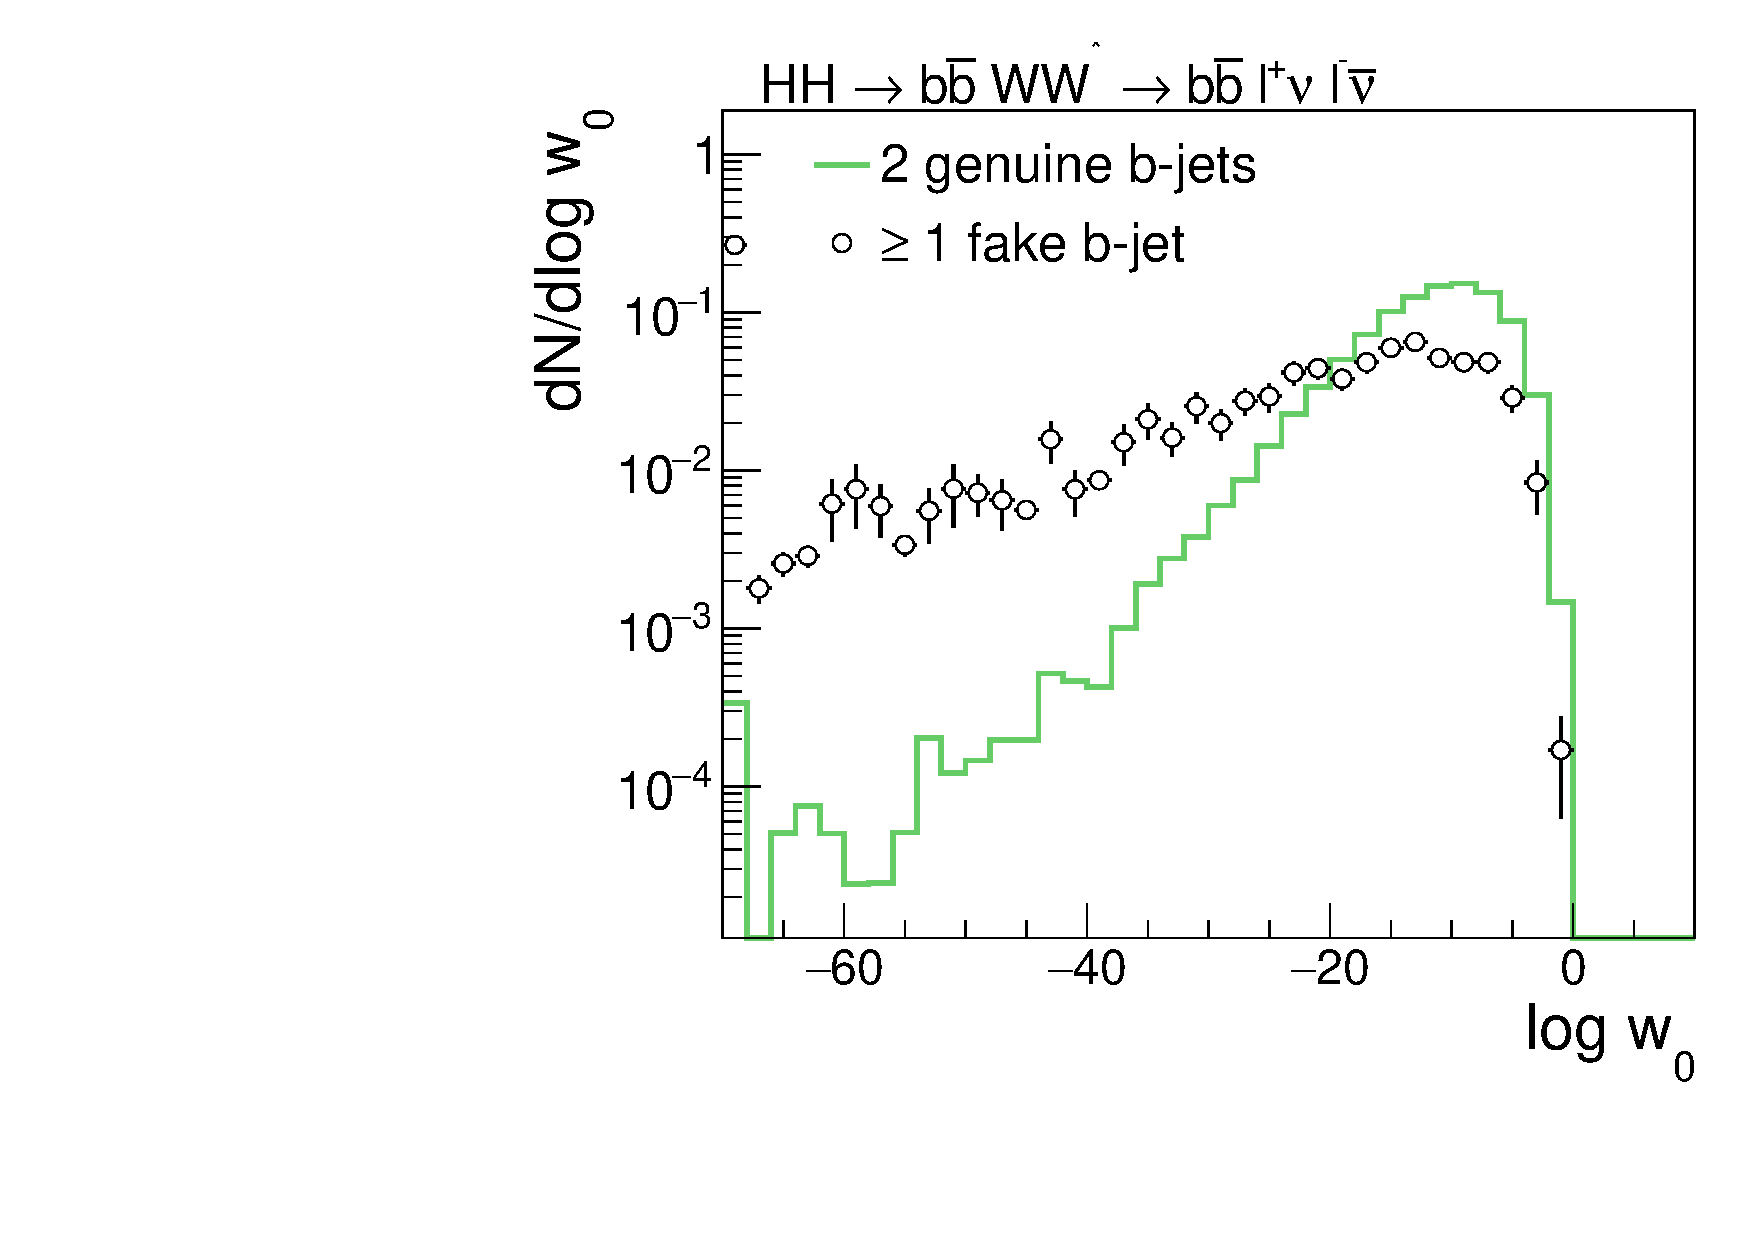
\includegraphics[width=0.48\textwidth]{plots/effectOfFakes_2histograms_probS_signal.pdf}
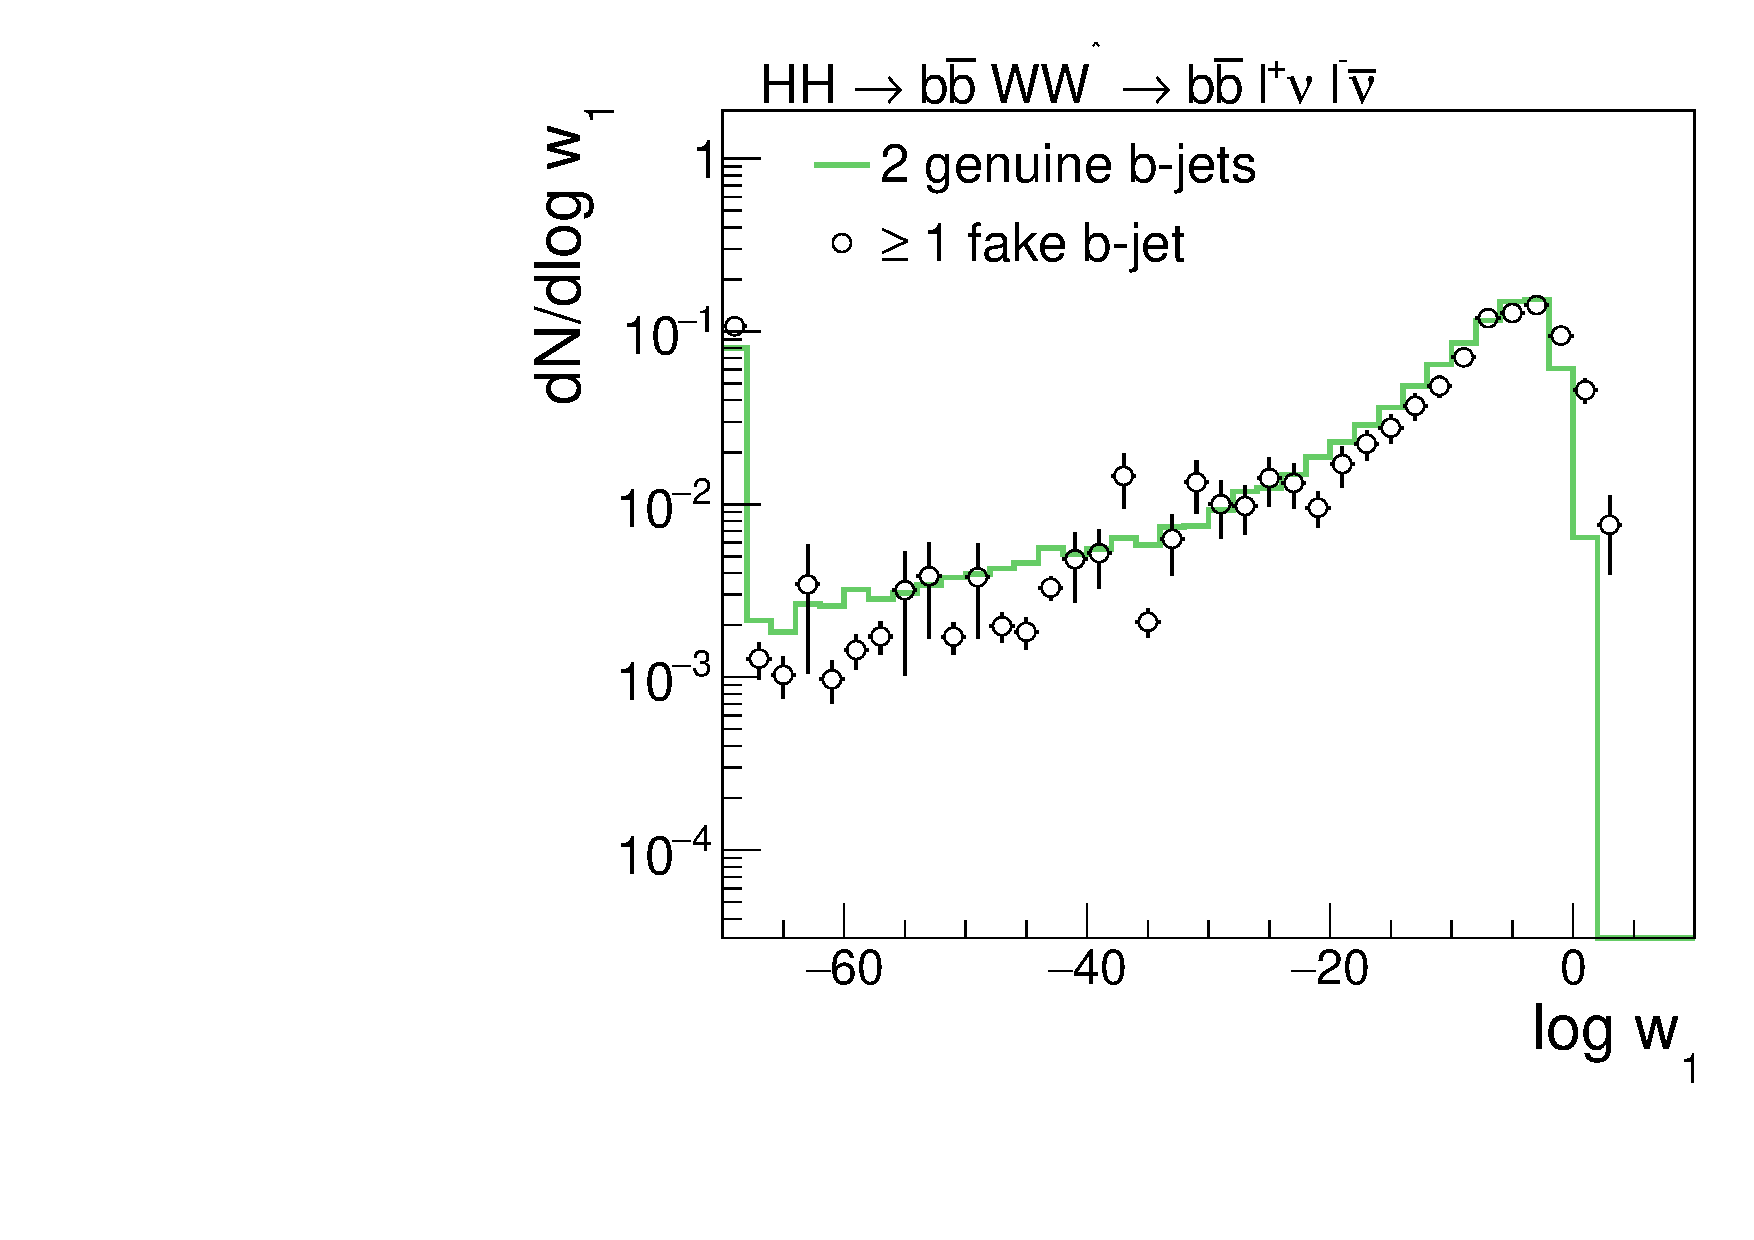
\includegraphics[width=0.48\textwidth]{plots/effectOfFakes_2histograms_probB_signal.pdf}
\hspace{0.04\textwidth}
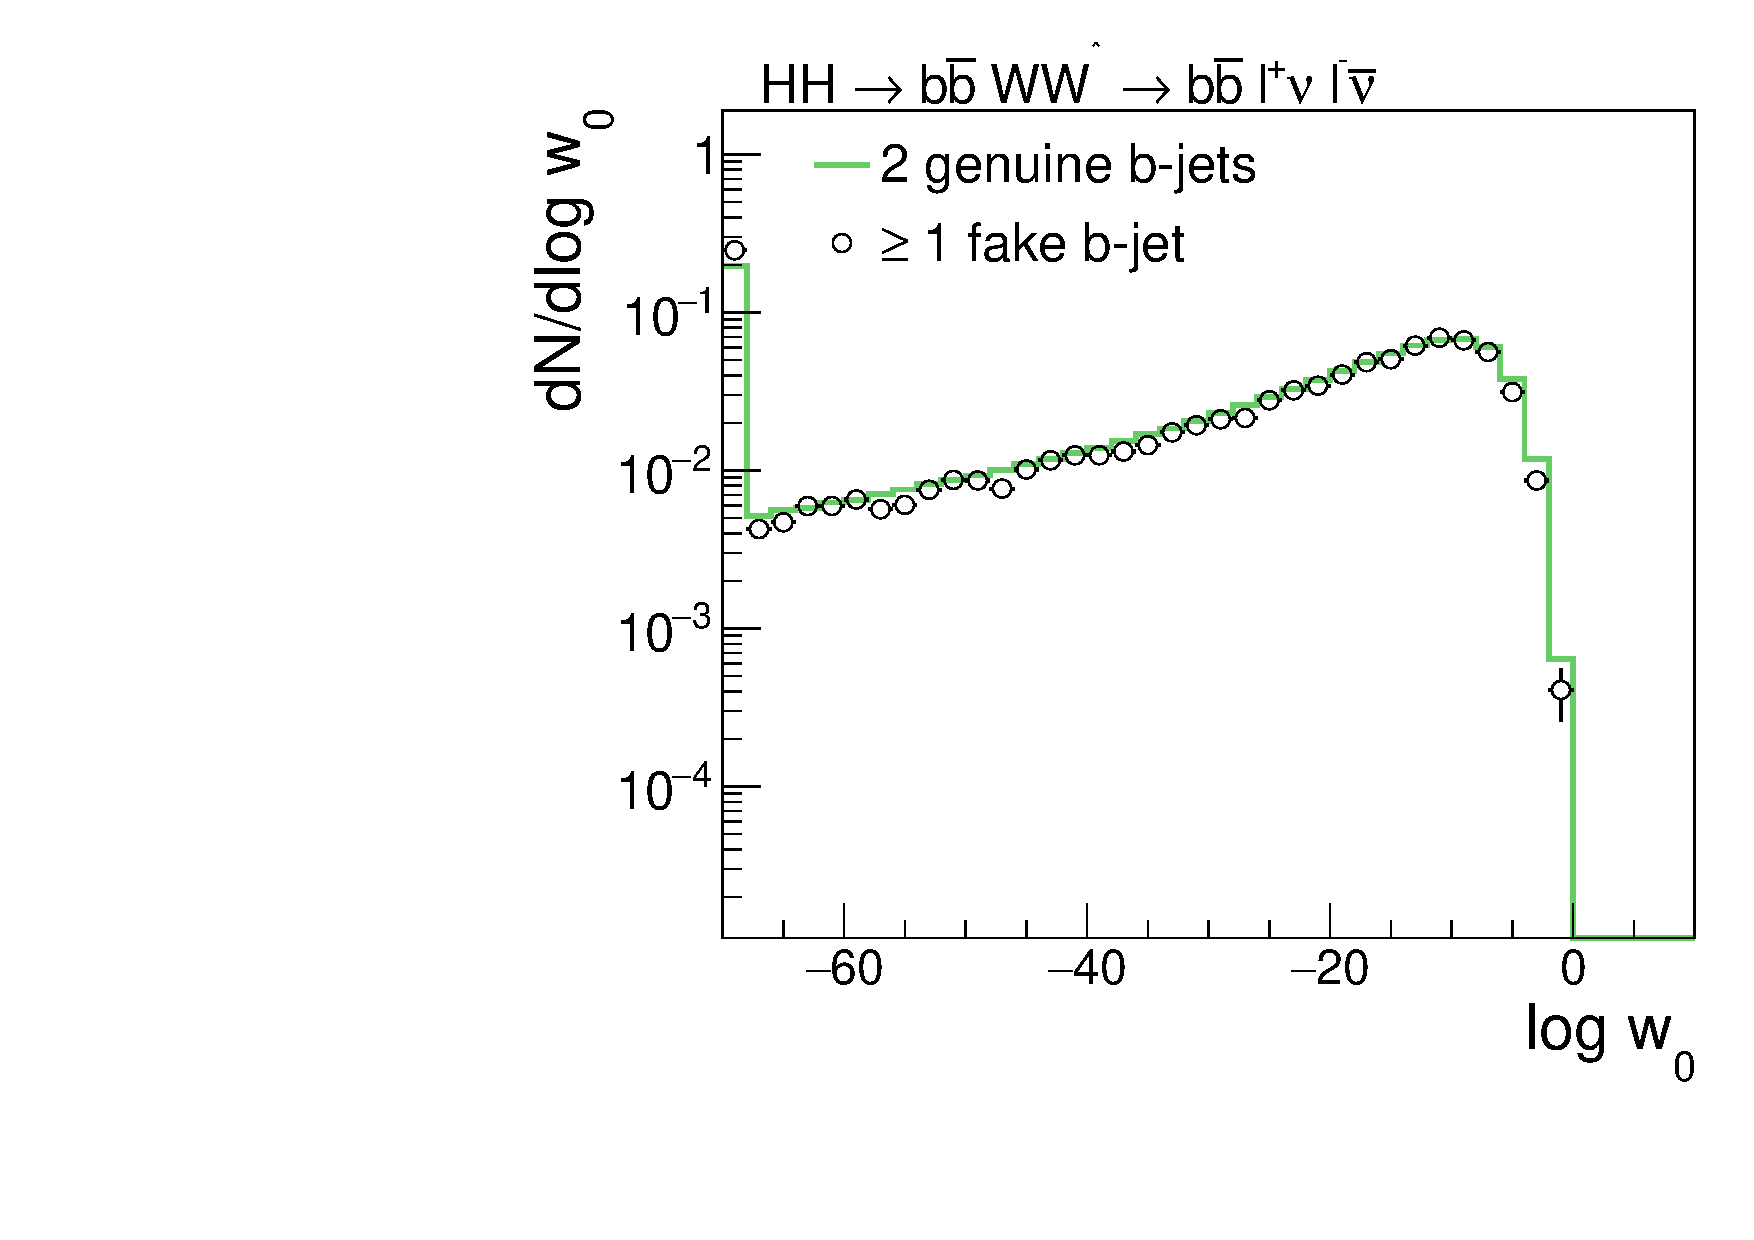
\includegraphics[width=0.48\textwidth]{plots/effectOfFakes_2histograms_probS_background.pdf}
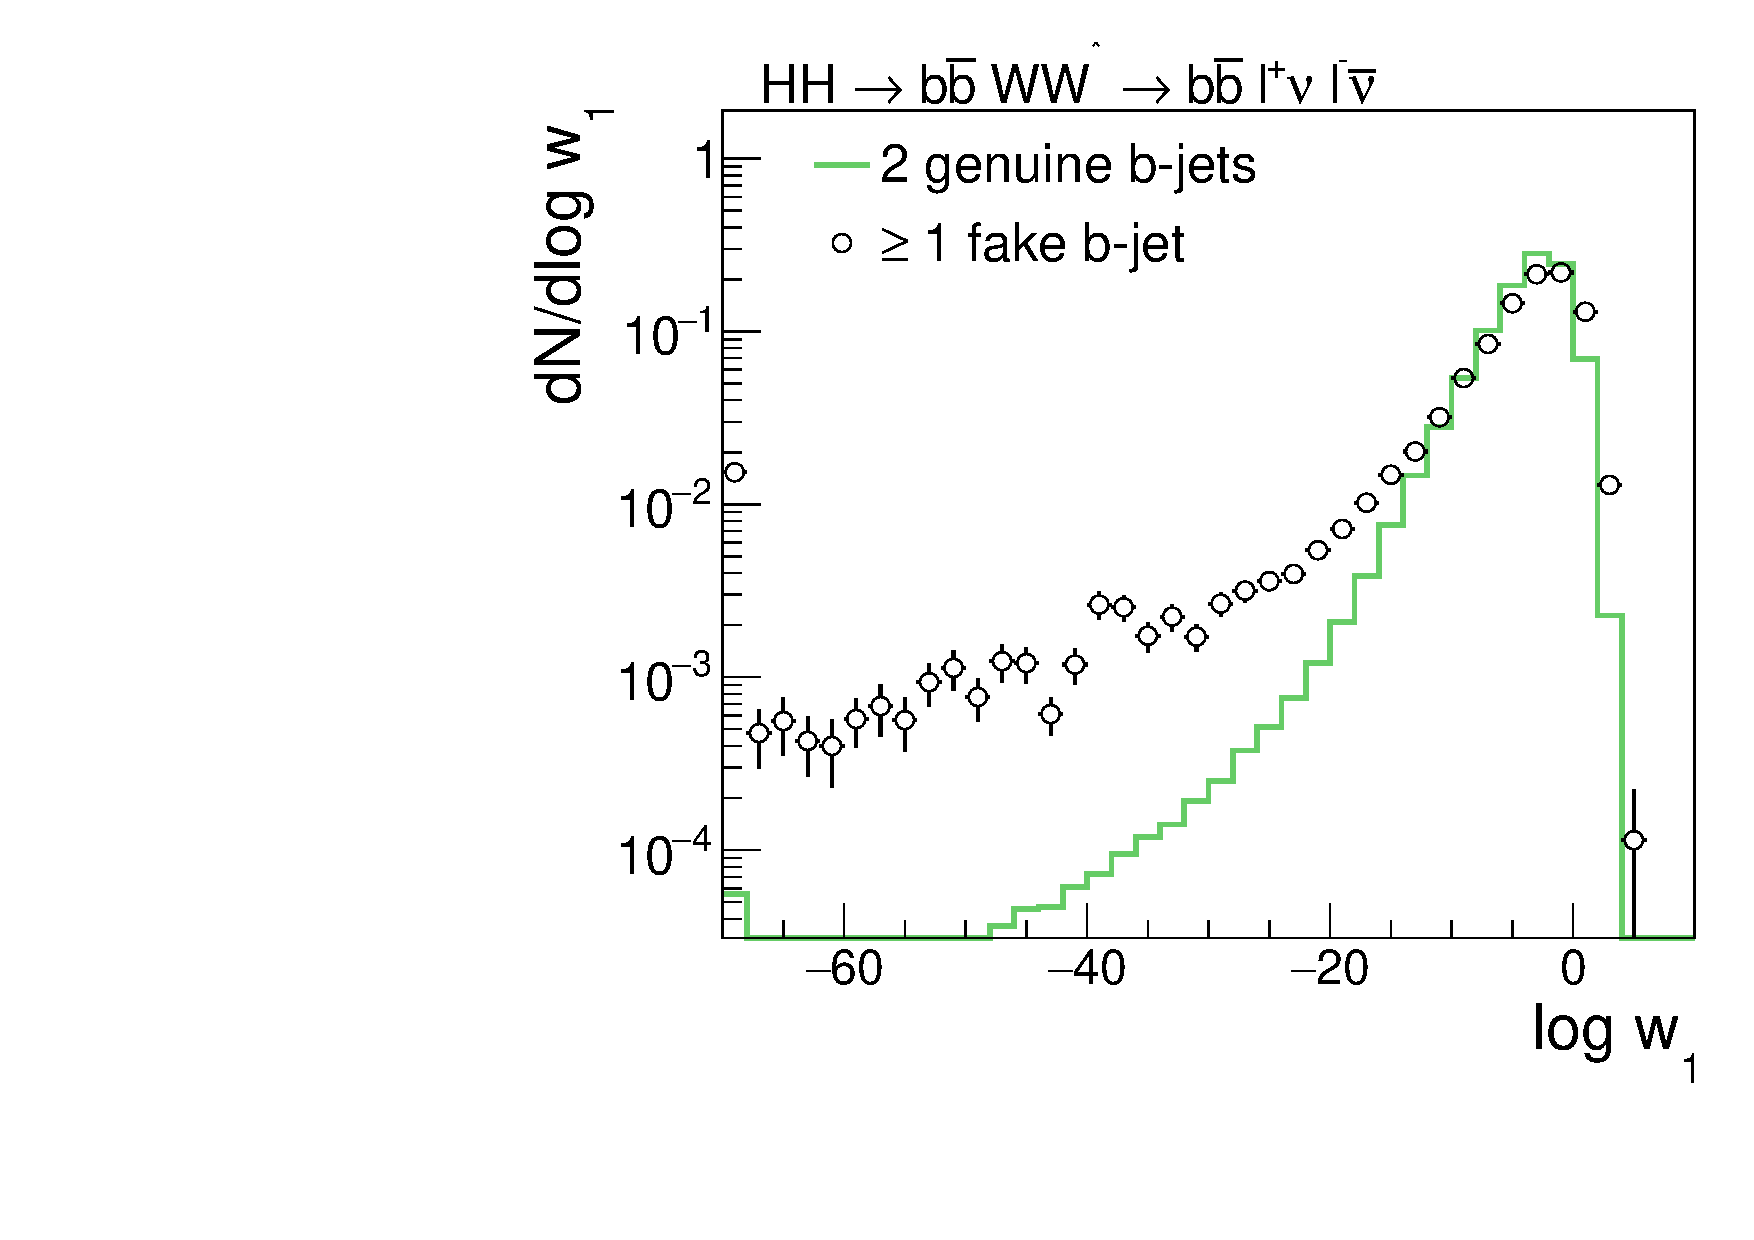
\includegraphics[width=0.48\textwidth]{plots/effectOfFakes_2histograms_probB_background.pdf}
\fi
\caption{
  Effect of misidentifying a light-quark or gluon jet (``fake'') as $\Pbottom$-jet candidate
  on the distribution in the probability densities $w_{0}(\vecy)$ (left) and $w_{1}(\vecy)$ (right)
  obtained for simulated $\dihiggs$ signal (top) and $\ttbar$ background (bottom) events.
}
\label{fig:probS_and_probB_fakeBJet}
\end{figure}

For a signal efficiency of $35\%$, the rate of $\ttbar$ background amounts to about $20\%$
in case a light-quark or gluon jet is misidentified as $\Pbottom$-jet.
This represents an increase in the $\ttbar$ background rate by about two orders of magnitude,
compared to the case that both $\Pbottom$-jets are genuine $\Pbottom$-jets.


\subsection{Mitigation of \texorpdfstring{$\Pbottom$}{b}-jet misidentification effect}

The degradation in the separation of the $\dihiggs$ signal from the $\ttbar$ background can be mitigated 
by marginalizing the expressions for the PDs $w_{0}(\vecy)$ and $w_{1}(\vecy)$ in Eqs.~(\ref{eq:mem_signal}) and~(\ref{eq:mem_background}),
assuming that one of the two true $\Pbottom$-jets failed to get reconstructed.
Marginalization means that the $\Pbottom$-jet variables $E_{\Pbottom}$, $\theta_{\Pbottom}$, and $\phi_{\Pbottom}$
are no longer used in the RHS of these expressions but instead integrated over:
\begin{linenowrapper}
\begin{equation*}
w_{i,\textrm{m}}(\vecy') = \int \, dE_{\Pbottom} \, d\theta_{\Pbottom} \, d\phi_{\Pbottom} \, w_{i}(\vecy) \, ,
\end{equation*}
\end{linenowrapper}
where we have added a subscript $m$ to denote the marginalized PDs and the vector $\vecy'$ equals the vector $\vecy$,
except that the variables $E_{\Pbottom}$, $\theta_{\Pbottom}$, and $\phi_{\Pbottom}$ are absent in the vector $\vecy'$.
Since we do not know whether the jet corresponding to the $\Pbottom$ quark or the one corresponding to the $\APbottom$ quark is the misidentified jet,
we perform the marginalization once with respect to the variables $E_{\Pbottom}$, $\theta_{\Pbottom}$, and $\phi_{\Pbottom}$ 
and once with respect to the variables $E_{\APbottom}$, $\theta_{\APbottom}$, and $\phi_{\APbottom}$ and take the sum.
The computing time required to evaluate the marginalized PDs $w_{0,\textrm{m}}(\vecy')$ and $w_{1,\textrm{m}}(\vecy')$
is similar to the time required to compute the un-marginalized PDs $w_{0}(\vecy')$ and $w_{1}(\vecy')$,
except for the factor two increase that results from the need to perform the marginalization with respect to the $\Pbottom$ and with respect to the $\APbottom$ quark.
The distributions in the marginalized LR $P_{\textrm{m}}(\vecy)$ obtained for the $\dihiggs$ signal as well as for the $\ttbar$ background 
and the corresponding ROC curve is shown in Fig.~\ref{fig:memLR_and_ROC_missingBJet}.
Marginalization reduces the amount of kinematic information, which is utilized for separating the signal from the background,
resulting in an increased overlap in the distributions in $P_{\textrm{m}}(\vecy)$ for the $\dihiggs$ signal and for the $\ttbar$ background,
but also makes the distributions less susceptible to the case that one of the true $\Pbottom$-jets fails to get reconstructed
and a light-quark or gluon jet is misidentified as $\Pbottom$-jet.

\begin{figure}
\ifx\ver\verPreprint
\setlength{\unitlength}{1mm}
\begin{center}
\begin{picture}(160,66)(0,0)
\put(-1.0, 1.0){\mbox{\includegraphics*[height=66mm]
 {plots/effectOfFakes_memLR_missingBJet.pdf}}}
\put(80.0, 0.0){\mbox{\includegraphics*[height=67mm]
 {plots/effectOfFakes_ROC_missingBJet.pdf}}}
\end{picture}
\end{center}
\fi
\ifx\ver\verPAPER
\centering
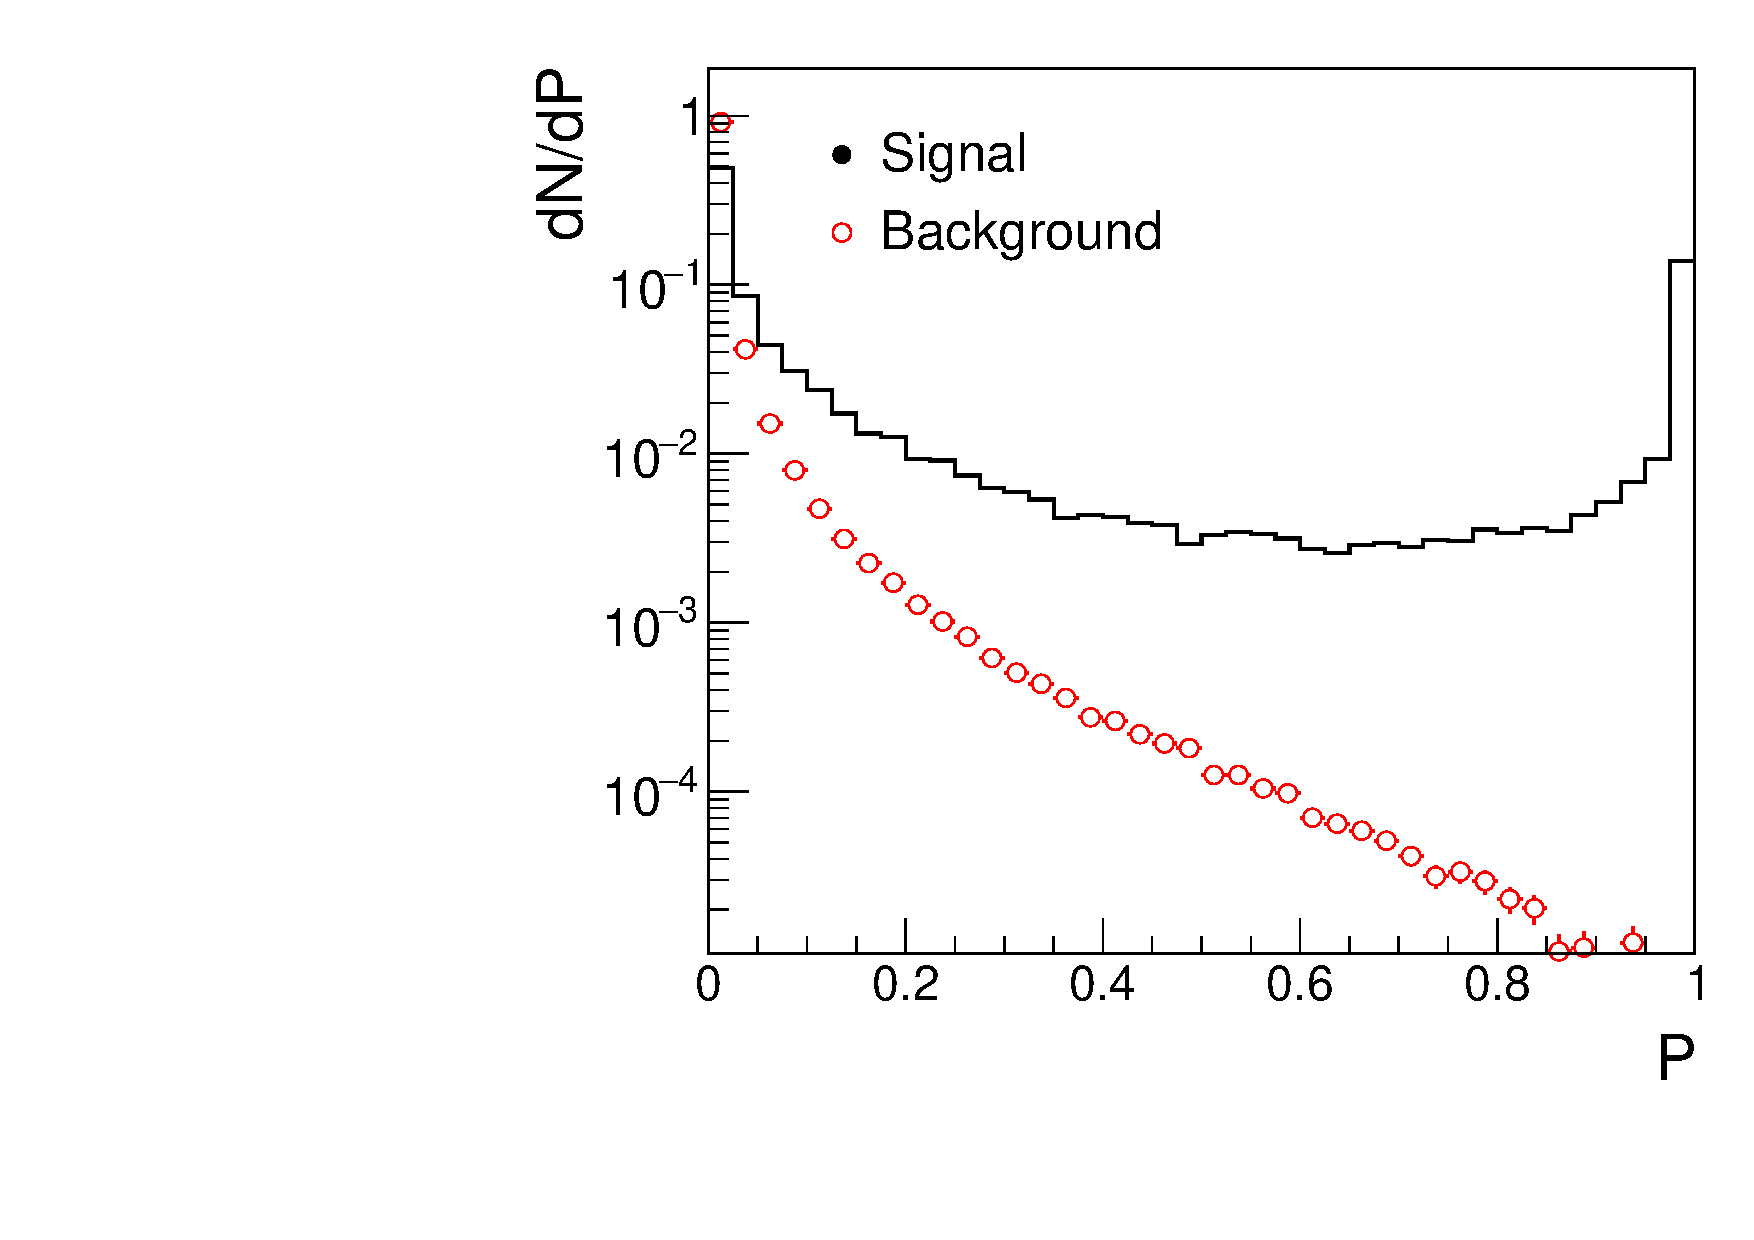
\includegraphics[width=0.48\textwidth]{plots/effectOfFakes_memLR_missingBJet.pdf}
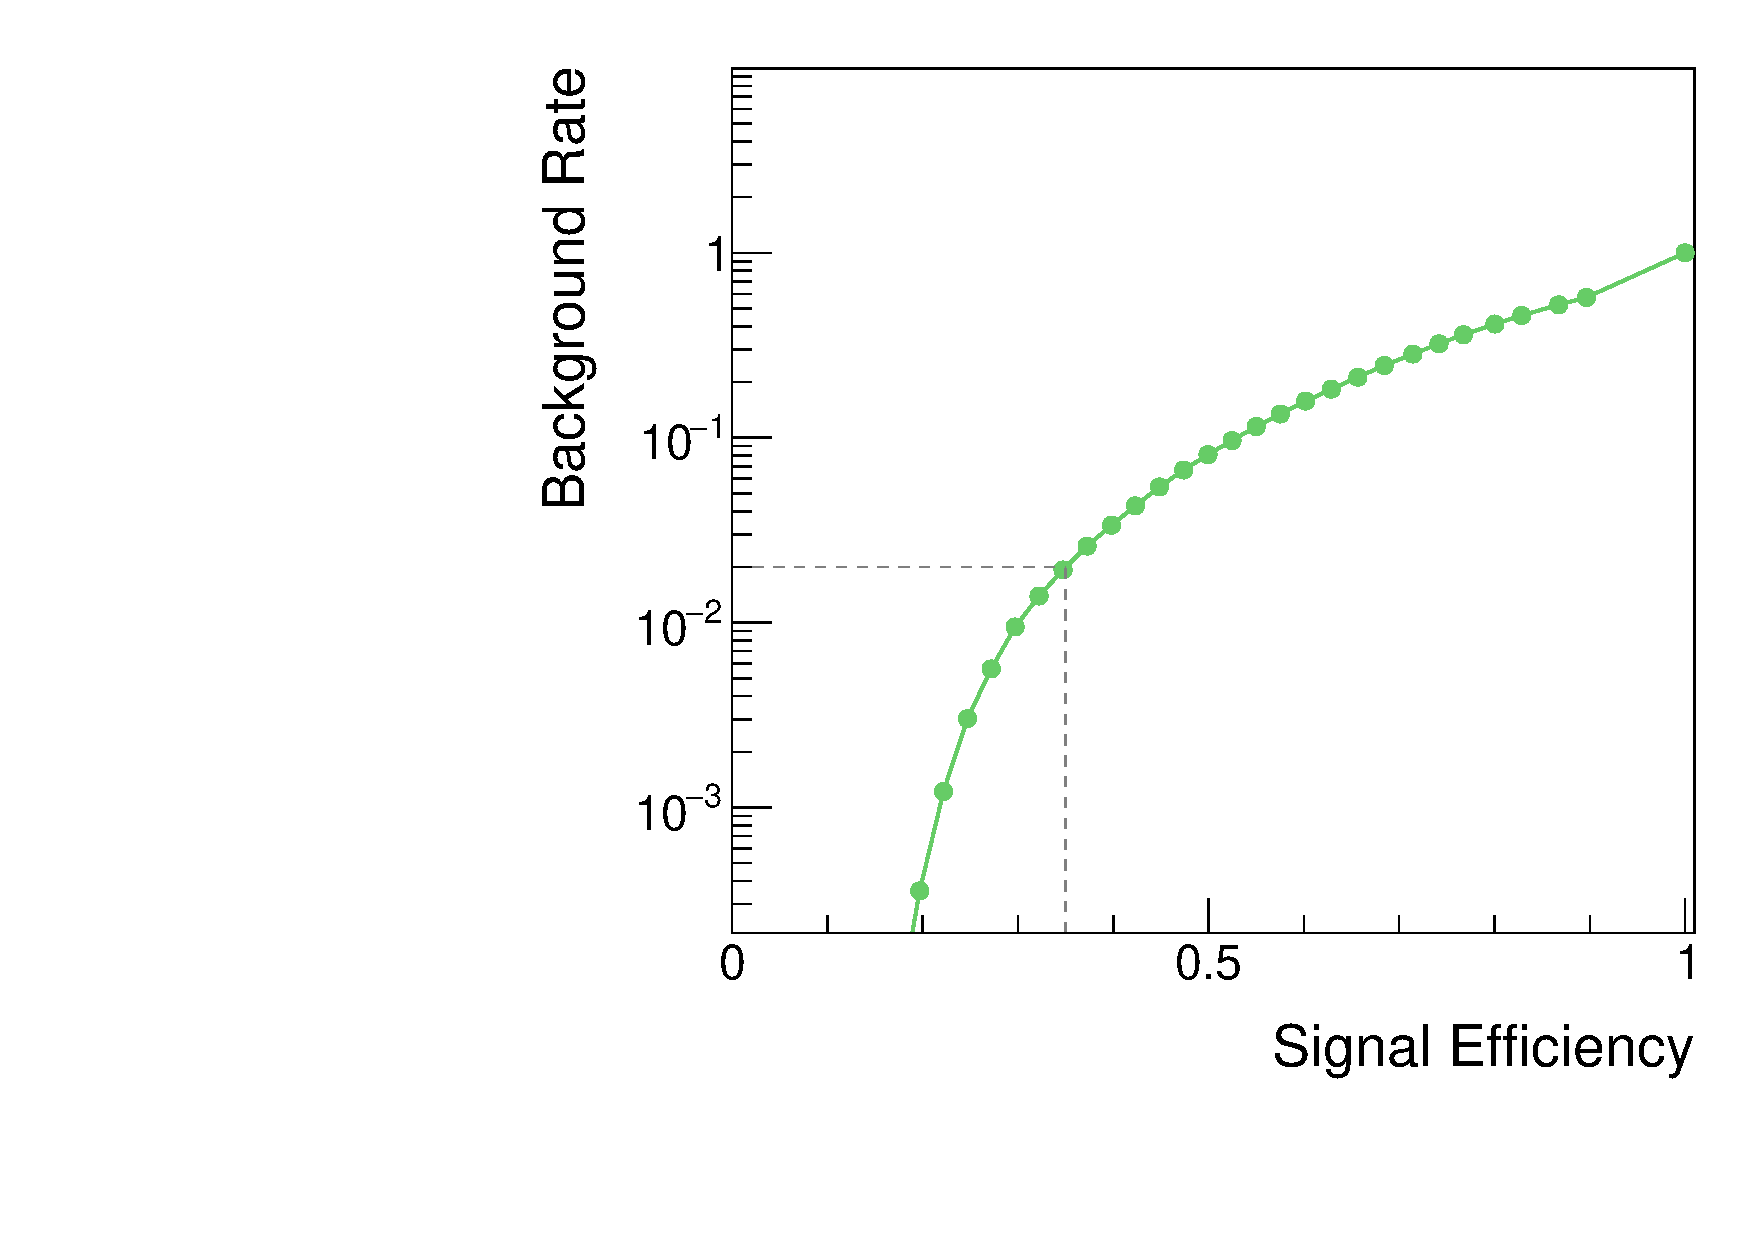
\includegraphics[width=0.48\textwidth]{plots/effectOfFakes_ROC_missingBJet.pdf}
\fi
\caption{
  Left: Distribution in the marginalized LR $P_{\textrm{m}}(\vecy)$, obtained for $\dihiggs$ signal and for $\ttbar$ background events.
  Right: Graph of background rate versus signal efficiency (``ROC curve''), obtained by applying a cut on the distribution shown on the left
  and varying the cut threshold.
}
\label{fig:memLR_and_ROC_missingBJet}
\end{figure}

Different options exist for using the marginalized LR $P_{\textrm{m}}(\vecy)$ in data analyses of $\dihiggs$ production at the LHC.
For instance, one may use the un-marginalized LR $P(\vecy)$ for events in which both reconstructed $\Pbottom$-jets pass tight $\Pbottom$-tagging criteria
and the marginalized LR $P_{\textrm{m}}(\vecy)$ for events in which one of the $\Pbottom$-jet candidate passes tight $\Pbottom$-tagging criteria,
while the other $\Pbottom$-jet candidate passes only loose $\Pbottom$-tagging criteria.
Alternatively, one may use the two-dimensional distribution in $P_{\textrm{m}}(\vecy)$ versus $P(\vecy)$ to separate the $\dihiggs$ signal from the $\ttbar$ background.
Yet another alternative is to use both likelihood ratios, $P_{\textrm{m}}(\vecy)$ and $P(\vecy)$,
as input to a machine-learning (ML) algorithm, for example a boosted decision tree~\cite{BDT} or an artificial neural network~\cite{ANN,chollet2015keras},
together with the $\Pbottom$-tagging discriminants of the two reconstructed $\Pbottom$-jet candidates and possibly other observables,
such as the total number of jets, the $\pT$ of the hadronic recoil, etc.
The CMS analysis of the associated production of a $\PHiggs$ boson with a top quark pair ($\Ptop\APtop\PHiggs$),
performed in the decay channel $\PHiggs \to \Pbottom\APbottom$ with the LHC Run $2$ data,
found that using the LR $P_{\textrm{m}}(\vecy)$ computed by the MEM as input to an ML algorithm
improved the signal-to-background separation compared to the case of either using the same ML algorithm without the LR $P_{\textrm{m}}(\vecy)$ as input
or of using the LR $P_{\textrm{m}}(\vecy)$ for the signal-to-background separation directly, without employing an ML algorithm~\cite{Sirunyan:2018mvw}.
The approach of using the LR $P_{\textrm{m}}(\vecy)$ as an input to an ML algorithm has the additional benefit
that other, subdominant, backgrounds can be included in the training of the ML algorithm, thereby further improving the sensitivity of the analysis.


\subsection{Effect of leading-order matrix elements}

The performance achieved in separating the $\dihiggs$ signal from the $\ttbar$ background
for MC samples simulated at LO and at NLO accuracy is shown in Fig.~\ref{fig:memLR_LO_vs_NLO}.
The signal and background events are studied on MC-truth level, assuming an optimal experimental resolution,
and are selected by requiring that both $\Pbottom$-jets are genuine $\Pbottom$-jets.
The corresponding ROC curve is presented in Fig.~\ref{fig:ROC_LO_vs_NLO}.
The usage of LO ME causes a moderate loss in the separation of the $\dihiggs$ signal from the $\ttbar$ background,
amounting to a few percent loss in signal efficiency (for the same background rate).

\begin{figure}
\ifx\ver\verPreprint
\setlength{\unitlength}{1mm}
\begin{center}
\begin{picture}(160,78)(0,0)
\put(0.0, 0.0){\mbox{\includegraphics*[height=78mm]
 {plots/lo_vs_nlo_memLR_signal.pdf}}}
\put(81.0, 0.0){\mbox{\includegraphics*[height=78mm]
 {plots/lo_vs_nlo_memLR_background.pdf}}}
\end{picture}
\end{center}
\fi
\ifx\ver\verPAPER
\centering
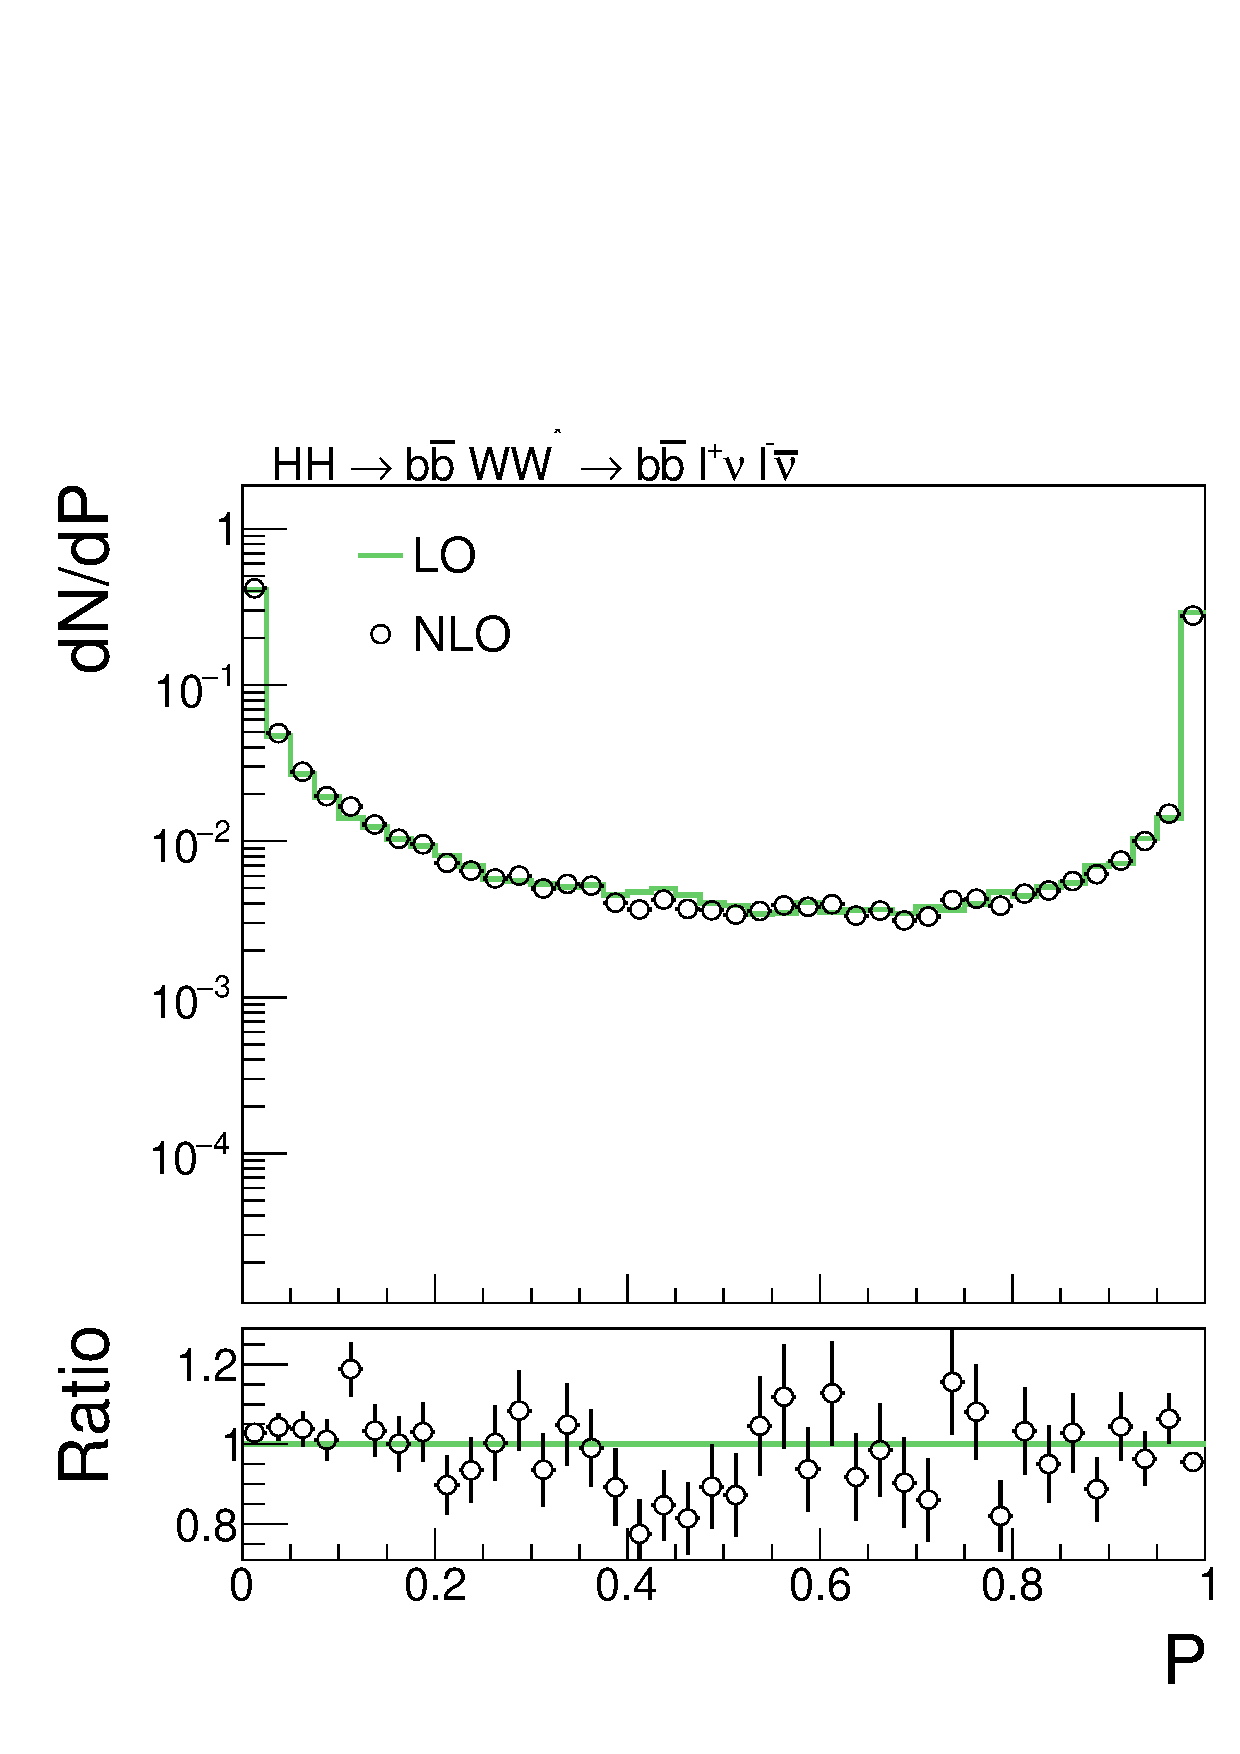
\includegraphics[width=0.48\textwidth]{plots/lo_vs_nlo_memLR_signal.pdf}
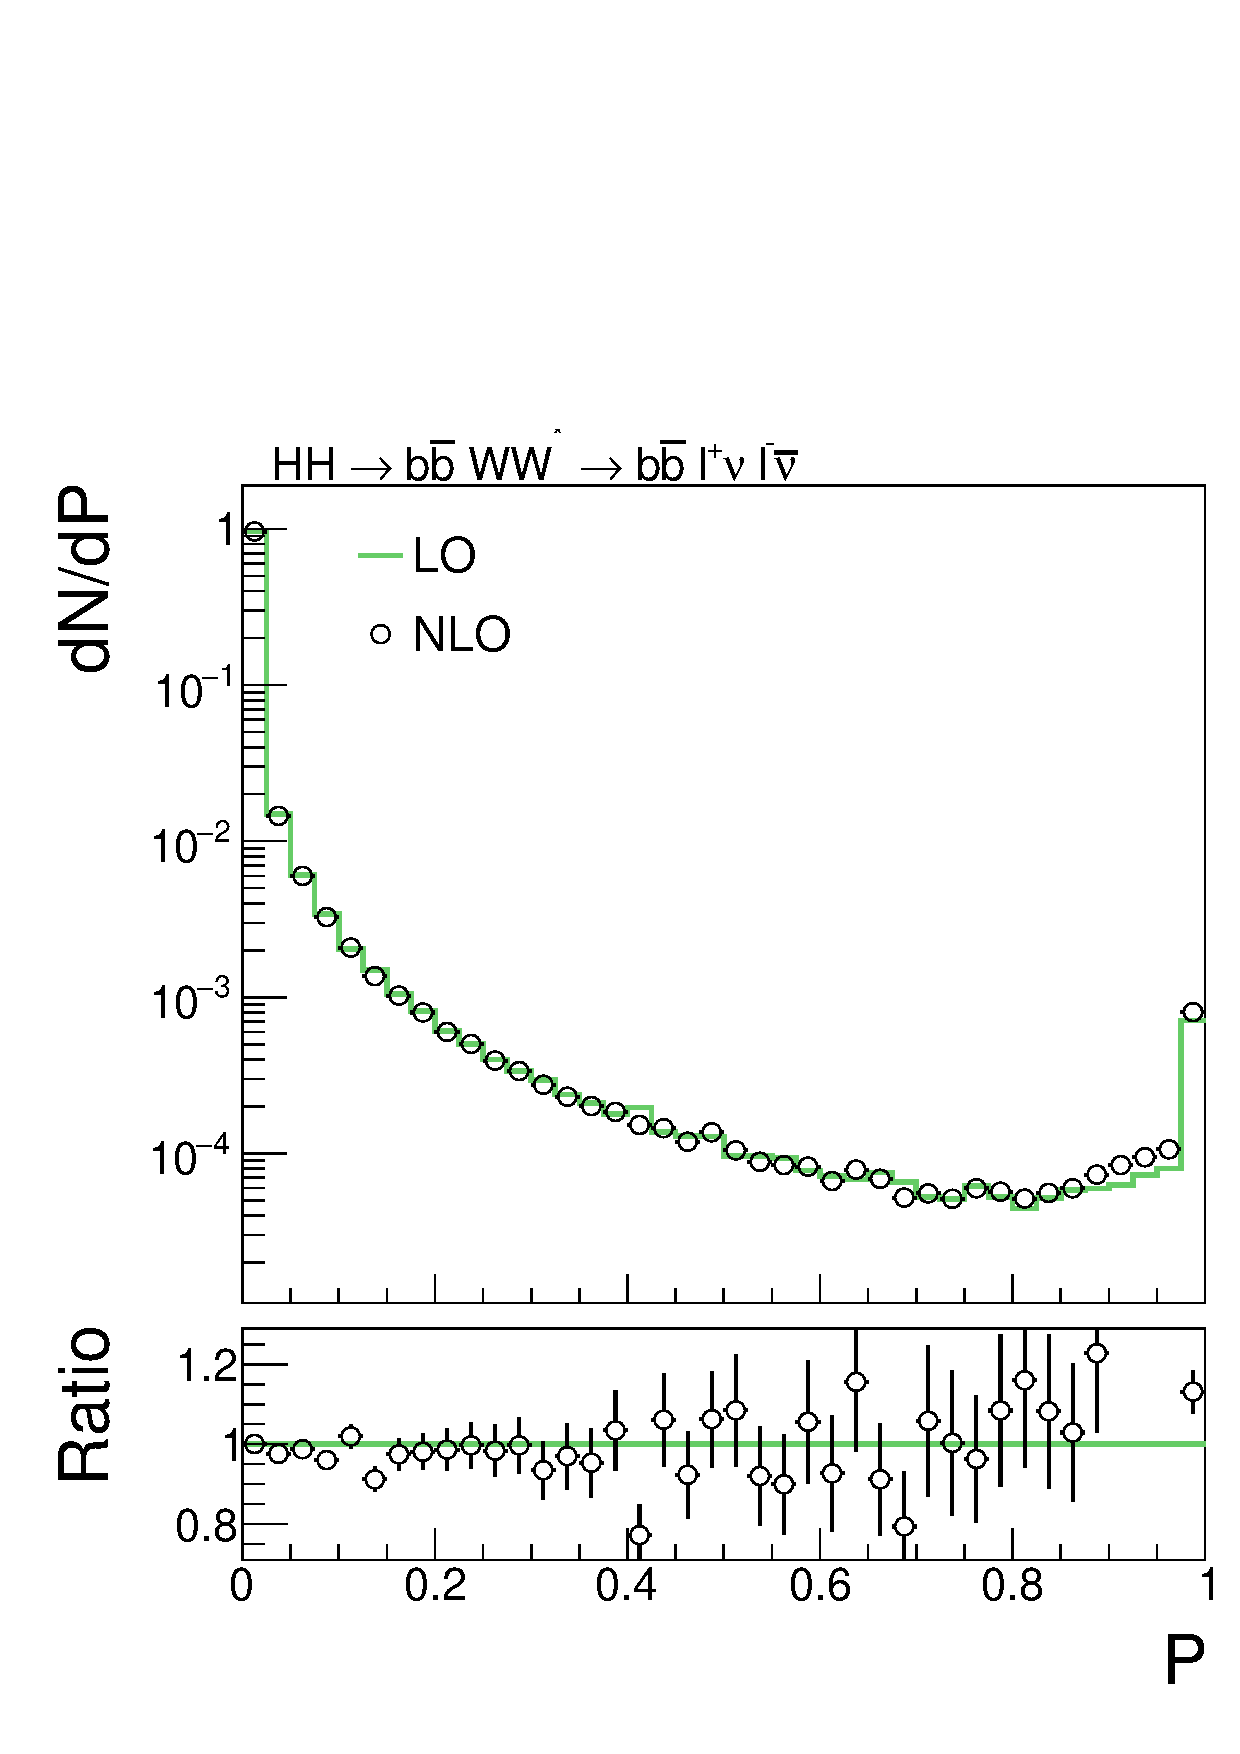
\includegraphics[width=0.48\textwidth]{plots/lo_vs_nlo_memLR_background.pdf}
\fi
\caption{
  Distribution in the LR $P(\vecy)$ 
  for $\dihiggs$ signal (left) and $\ttbar$ background (right) events
  simulated at LO and at NLO accuracy in pQCD.
  The signal and background events are studied on MC-truth level
  and are selected by requiring that both $\Pbottom$-jets are genuine $\Pbottom$-jets.
}
\label{fig:memLR_LO_vs_NLO}
\end{figure}

\begin{figure}
\ifx\ver\verPreprint
\setlength{\unitlength}{1mm}
\begin{center}
\begin{picture}(160,67)(0,0)
\put(39.5, 0.0){\mbox{\includegraphics*[height=67mm]
 {plots/lo_vs_nlo_ROC.pdf}}}
\end{picture}
\end{center}
\fi
\ifx\ver\verPAPER
\centering
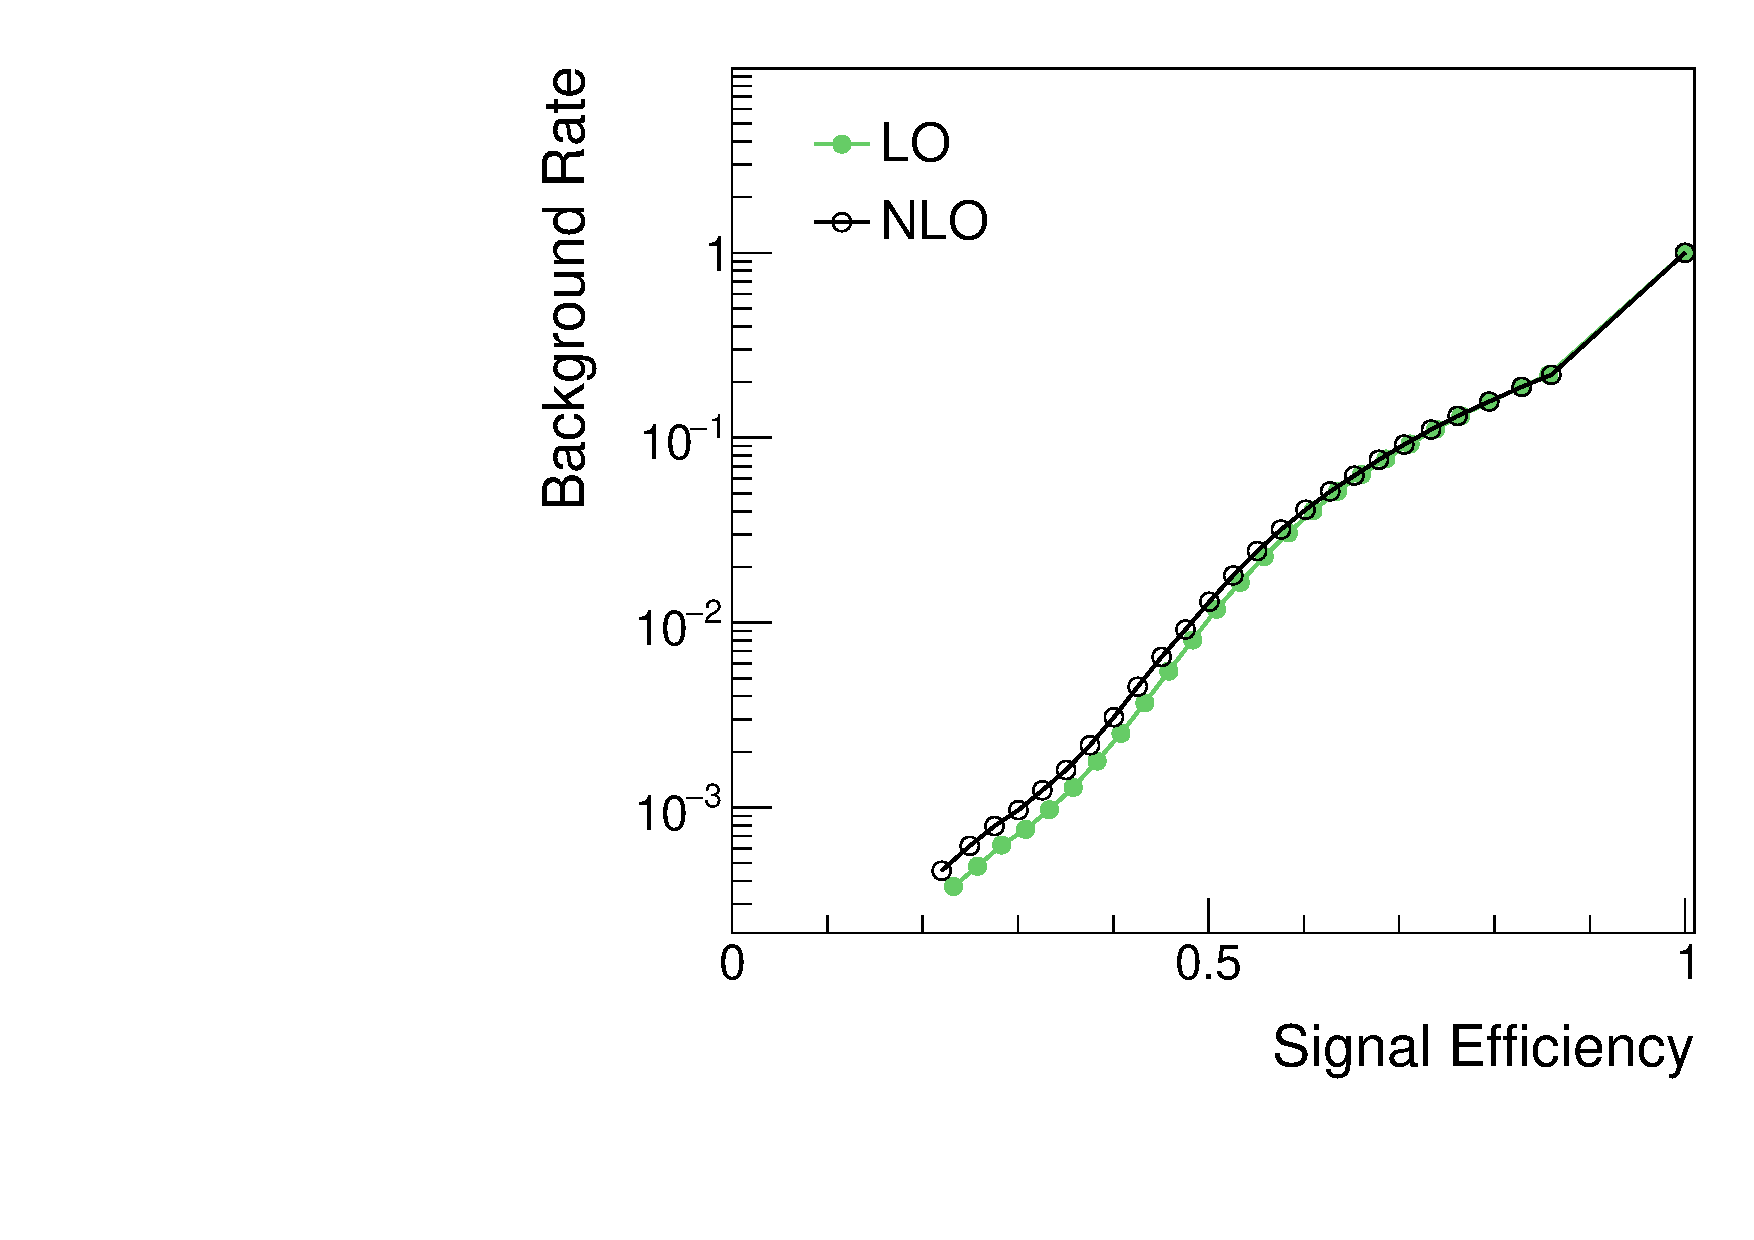
\includegraphics[width=0.48\textwidth]{plots/lo_vs_nlo_ROC.pdf}
\fi
\caption{
  Separation between the $\dihiggs$ signal and the $\ttbar$ background 
  for events simulated at LO and at NLO accuracy in pQCD.
  The signal and background events are studied on MC-truth level
  and are selected by requiring that both $\Pbottom$-jets are genuine $\Pbottom$-jets.
}
\label{fig:ROC_LO_vs_NLO}
\end{figure}


\subsection{Computing-time requirements of the MEM}
\label{sec:computing_time_requirements}

One remaining issue in practical applications of the MEM may be the computing time requirements.
Experimental analyses will usually need to evaluate the integrals given by Eqs.~(\ref{eq:mem_signal}) and~(\ref{eq:mem_background})
multiple times for each event in order to assess the effect of systematic uncertainties.
Taken together with the large cross section for $\ttbar$ production at the LHC,
the integrals in Eqs.~(\ref{eq:mem_signal}) and~(\ref{eq:mem_background}) may need to be computed in the order of $100$ million times.
Even with several thousands of computing jobs running in parallel,
as it is nowadays commonplace for experimental data analyses performed at the LHC,
the computation still requires a few weeks of nonstop computing time.
Several possibilities to speed up the numeric integrations, which take most of the computing time in practical applications of the MEM,
have been explored in the literature.
One alternative is to use vector integrands to evaluate the likelihood ratio for all systematic uncertainties simultaneously~\cite{CUBA},
taking advantage of the fact that the systematic uncertainties typically constitute small changes with respect to the nominal value.
Another alternative is to take advantage of the parallelizability of multidimensional integration and perform the integration on graphics processing units (GPUs).
Speedup factors of order $100$, compared to using a single core of a general-purpose central processing unit (CPU) 
such as the $2.30$~GHz Intel\TReg~Xeon\TReg~E5-2695V3 processor that we used for the studies presented in this paper,
are reported in the literature for performing numeric integrations on GPUs~\cite{Hagiwara:2009aq,Hagiwara:2009cy,Kanzaki:2010ym,Hagiwara:2013oka,Schouten:2014yza,Grasseau:2015vfa}.
